\PassOptionsToPackage{unicode=true}{hyperref} % options for packages loaded elsewhere
\PassOptionsToPackage{hyphens}{url}
\PassOptionsToPackage{dvipsnames,svgnames*,x11names*}{xcolor}
%
\documentclass[12pt,krantz2]{krantz}
\usepackage{lmodern}
\usepackage{amssymb,amsmath}
\usepackage{ifxetex,ifluatex}
\usepackage{fixltx2e} % provides \textsubscript
\ifnum 0\ifxetex 1\fi\ifluatex 1\fi=0 % if pdftex
  \usepackage[T1]{fontenc}
  \usepackage[utf8]{inputenc}
  \usepackage{textcomp} % provides euro and other symbols
\else % if luatex or xelatex
  \usepackage{unicode-math}
  \defaultfontfeatures{Ligatures=TeX,Scale=MatchLowercase}
    \setmonofont[Mapping=tex-ansi,Scale=0.65]{Source Code Pro}
\fi
% use upquote if available, for straight quotes in verbatim environments
\IfFileExists{upquote.sty}{\usepackage{upquote}}{}
% use microtype if available
\IfFileExists{microtype.sty}{%
\usepackage[]{microtype}
\UseMicrotypeSet[protrusion]{basicmath} % disable protrusion for tt fonts
}{}
\IfFileExists{parskip.sty}{%
\usepackage{parskip}
}{% else
\setlength{\parindent}{0pt}
\setlength{\parskip}{6pt plus 2pt minus 1pt}
}
\usepackage{xcolor}
\usepackage{hyperref}
\hypersetup{
            pdftitle={HealthyR: R for health data analysis},
            pdfauthor={Ewen Harrison and Riinu Ots},
            colorlinks=true,
            linkcolor=Maroon,
            filecolor=Maroon,
            citecolor=Blue,
            urlcolor=Blue,
            breaklinks=true}
\urlstyle{same}  % don't use monospace font for urls
\usepackage{color}
\usepackage{fancyvrb}
\newcommand{\VerbBar}{|}
\newcommand{\VERB}{\Verb[commandchars=\\\{\}]}
\DefineVerbatimEnvironment{Highlighting}{Verbatim}{commandchars=\\\{\}}
% Add ',fontsize=\small' for more characters per line
\usepackage{framed}
\definecolor{shadecolor}{RGB}{248,248,248}
\newenvironment{Shaded}{\begin{snugshade}}{\end{snugshade}}
\newcommand{\AlertTok}[1]{\textcolor[rgb]{0.94,0.16,0.16}{#1}}
\newcommand{\AnnotationTok}[1]{\textcolor[rgb]{0.56,0.35,0.01}{\textbf{\textit{#1}}}}
\newcommand{\AttributeTok}[1]{\textcolor[rgb]{0.77,0.63,0.00}{#1}}
\newcommand{\BaseNTok}[1]{\textcolor[rgb]{0.00,0.00,0.81}{#1}}
\newcommand{\BuiltInTok}[1]{#1}
\newcommand{\CharTok}[1]{\textcolor[rgb]{0.31,0.60,0.02}{#1}}
\newcommand{\CommentTok}[1]{\textcolor[rgb]{0.56,0.35,0.01}{\textit{#1}}}
\newcommand{\CommentVarTok}[1]{\textcolor[rgb]{0.56,0.35,0.01}{\textbf{\textit{#1}}}}
\newcommand{\ConstantTok}[1]{\textcolor[rgb]{0.00,0.00,0.00}{#1}}
\newcommand{\ControlFlowTok}[1]{\textcolor[rgb]{0.13,0.29,0.53}{\textbf{#1}}}
\newcommand{\DataTypeTok}[1]{\textcolor[rgb]{0.13,0.29,0.53}{#1}}
\newcommand{\DecValTok}[1]{\textcolor[rgb]{0.00,0.00,0.81}{#1}}
\newcommand{\DocumentationTok}[1]{\textcolor[rgb]{0.56,0.35,0.01}{\textbf{\textit{#1}}}}
\newcommand{\ErrorTok}[1]{\textcolor[rgb]{0.64,0.00,0.00}{\textbf{#1}}}
\newcommand{\ExtensionTok}[1]{#1}
\newcommand{\FloatTok}[1]{\textcolor[rgb]{0.00,0.00,0.81}{#1}}
\newcommand{\FunctionTok}[1]{\textcolor[rgb]{0.00,0.00,0.00}{#1}}
\newcommand{\ImportTok}[1]{#1}
\newcommand{\InformationTok}[1]{\textcolor[rgb]{0.56,0.35,0.01}{\textbf{\textit{#1}}}}
\newcommand{\KeywordTok}[1]{\textcolor[rgb]{0.13,0.29,0.53}{\textbf{#1}}}
\newcommand{\NormalTok}[1]{#1}
\newcommand{\OperatorTok}[1]{\textcolor[rgb]{0.81,0.36,0.00}{\textbf{#1}}}
\newcommand{\OtherTok}[1]{\textcolor[rgb]{0.56,0.35,0.01}{#1}}
\newcommand{\PreprocessorTok}[1]{\textcolor[rgb]{0.56,0.35,0.01}{\textit{#1}}}
\newcommand{\RegionMarkerTok}[1]{#1}
\newcommand{\SpecialCharTok}[1]{\textcolor[rgb]{0.00,0.00,0.00}{#1}}
\newcommand{\SpecialStringTok}[1]{\textcolor[rgb]{0.31,0.60,0.02}{#1}}
\newcommand{\StringTok}[1]{\textcolor[rgb]{0.31,0.60,0.02}{#1}}
\newcommand{\VariableTok}[1]{\textcolor[rgb]{0.00,0.00,0.00}{#1}}
\newcommand{\VerbatimStringTok}[1]{\textcolor[rgb]{0.31,0.60,0.02}{#1}}
\newcommand{\WarningTok}[1]{\textcolor[rgb]{0.56,0.35,0.01}{\textbf{\textit{#1}}}}
\usepackage{longtable,booktabs}
% Fix footnotes in tables (requires footnote package)
\IfFileExists{footnote.sty}{\usepackage{footnote}\makesavenoteenv{longtable}}{}
\usepackage{graphicx,grffile}
\makeatletter
\def\maxwidth{\ifdim\Gin@nat@width>\linewidth\linewidth\else\Gin@nat@width\fi}
\def\maxheight{\ifdim\Gin@nat@height>\textheight\textheight\else\Gin@nat@height\fi}
\makeatother
% Scale images if necessary, so that they will not overflow the page
% margins by default, and it is still possible to overwrite the defaults
% using explicit options in \includegraphics[width, height, ...]{}
\setkeys{Gin}{width=\maxwidth,height=\maxheight,keepaspectratio}
\setlength{\emergencystretch}{3em}  % prevent overfull lines
\providecommand{\tightlist}{%
  \setlength{\itemsep}{0pt}\setlength{\parskip}{0pt}}
\setcounter{secnumdepth}{5}
% Redefines (sub)paragraphs to behave more like sections
\ifx\paragraph\undefined\else
\let\oldparagraph\paragraph
\renewcommand{\paragraph}[1]{\oldparagraph{#1}\mbox{}}
\fi
\ifx\subparagraph\undefined\else
\let\oldsubparagraph\subparagraph
\renewcommand{\subparagraph}[1]{\oldsubparagraph{#1}\mbox{}}
\fi

% set default figure placement to htbp
\makeatletter
\def\fps@figure{htbp}
\makeatother

\usepackage{booktabs}
\usepackage{longtable}
\usepackage[bf,singlelinecheck=off]{caption}

% Required for kableExtra - EMH 29/07/2019
\usepackage{array}
\usepackage{multirow}
% \usepackage[table]{xcolor} %This conflicted
\usepackage{wrapfig}
\usepackage{float}
\usepackage{colortbl}
\usepackage{pdflscape}
\usepackage{tabu}
\usepackage{threeparttable}
\usepackage[normalem]{ulem}

% Changing line spacing of verbatim (R code results) - RO
% Should only be temp fix, as all verbatim affect including
% chapter numbers, titles, quotes etc - EH
\usepackage{etoolbox}
\BeforeBeginEnvironment{verbatim}{\def\baselinestretch{0.7}}

% To print text width - RO
% \printinunitsof{cm}\prntlen{\textwidth}
\usepackage{layouts}

% float handling package  - RO
\usepackage{placeins}

% krantz2 option - EMH 05/09/2019
% \documentclass[krantz2]{krantz}

\usepackage{framed,color}
\definecolor{shadecolor}{RGB}{248,248,248}

\renewcommand{\textfraction}{0.05}
\renewcommand{\topfraction}{0.8}
\renewcommand{\bottomfraction}{0.8}
\renewcommand{\floatpagefraction}{0.75}

\renewenvironment{quote}{\begin{VF}}{\end{VF}}
\let\oldhref\href
\renewcommand{\href}[2]{#2\footnote{\url{#1}}}

\makeatletter
\newenvironment{kframe}{%
\medskip{}
\setlength{\fboxsep}{.8em}
 \def\at@end@of@kframe{}%
 \ifinner\ifhmode%
  \def\at@end@of@kframe{\end{minipage}}%
  \begin{minipage}{\columnwidth}%
 \fi\fi%
 \def\FrameCommand##1{\hskip\@totalleftmargin \hskip-\fboxsep
 \colorbox{shadecolor}{##1}\hskip-\fboxsep
     % There is no \\@totalrightmargin, so:
     \hskip-\linewidth \hskip-\@totalleftmargin \hskip\columnwidth}%
 \MakeFramed {\advance\hsize-\width
   \@totalleftmargin\z@ \linewidth\hsize
   \@setminipage}}%
 {\par\unskip\endMakeFramed%
 \at@end@of@kframe}
\makeatother

\renewenvironment{Shaded}{\begin{kframe}}{\end{kframe}}

\usepackage{makeidx}
\makeindex

\urlstyle{tt}

\usepackage{amsthm}
\makeatletter
\def\thm@space@setup{%
  \thm@preskip=8pt plus 2pt minus 4pt
  \thm@postskip=\thm@preskip
}
\makeatother

\frontmatter
\usepackage{booktabs}
\usepackage{longtable}
\usepackage{array}
\usepackage{multirow}
\usepackage{wrapfig}
\usepackage{float}
\usepackage{colortbl}
\usepackage{pdflscape}
\usepackage{tabu}
\usepackage{threeparttable}
\usepackage{threeparttablex}
\usepackage[normalem]{ulem}
\usepackage{makecell}
\usepackage{xcolor}
\usepackage[]{natbib}
\bibliographystyle{apalike}

\title{HealthyR: R for health data analysis}
\author{Ewen Harrison and Riinu Ots}
\date{2020-01-27}

\begin{document}
\maketitle

% you may need to leave a few empty pages before the dedication page

%\cleardoublepage\newpage\thispagestyle{empty}\null
%\cleardoublepage\newpage\thispagestyle{empty}\null
%\cleardoublepage\newpage
\thispagestyle{empty}

\begin{center}
"The future is already here — it's just not very evenly distributed." - William Gibson
%\includegraphics{images/dedication.pdf}
\end{center}

\setlength{\abovedisplayskip}{-5pt}
\setlength{\abovedisplayshortskip}{-5pt}

{
\hypersetup{linkcolor=}
\setcounter{tocdepth}{2}
\tableofcontents
}
\listoftables
\listoffigures
\hypertarget{preface}{%
\chapter*{Preface}\label{preface}}


This is the electronic version of the HealthyR book that is published by CRC Press/Chapman \& Hall in summer 2020.
The electronic version will always be freely and fully available.

HealthyR resources: \href{https://healthyr.surgicalinformatics.org/}{healthyr.surgicalinformatics.orgs}

Version 0.9.7

This work is licensed under the Creative Commons Attribution-NonCommercial-NoDerivs 3.0 United States License. To view a copy of this license, visit \url{http://creativecommons.org/licenses/by-nc-nd/3.0/us/}

\hypertarget{why-read-this-book}{%
\section*{Why read this book}\label{why-read-this-book}}


\begin{quote}
We are drowning in information but starved for knowledge.\\
John Naisbitt
\end{quote}

In this age of information, the manipulation, analysis and interpretation of data has become paramount.
Nowhere more so than in the delivery of healthcare.
From the understanding of disease and the development of new treatments, to the diagnosis and management of individual patients, the use of data and technology is now an integral part of the business of healthcare.

Those working in healthcare interact daily with data, often without realising it.
The conversion of this avalanche of information to useful knowledge is essential for high quality patient care.
An important part of this information revolution is the opportunity for everybody to become involved in data analysis.
This democratisation of data analysis is driven in part by the open source software movement -- no longer do we require expensive specialised software to do this.

The statistical programming language, R, is firmly at the heart of this!

This book will take an individual with little or no experience in data analysis all the way through to performing sophisticated analyses.
We emphasise the importance of understanding the underlying data with liberal use of plotting, rather than relying on opaque and possibly poorly understand statistical tests.
There are numerous examples included that can be adapted for your own data, together with our own R packages with easy-to-use functions.

We have a lot of fun teaching this course and focus on making the material as accessible as possible.
We banish equations in favour of code and use examples rather than lengthy explanations.
We are grateful to the many individuals and students who have helped refine these and welcome suggestions and bug reports via \url{https://github.com/SurgicalInformatics}.

Ewen Harrison and Riinu Ots

August 2019

\hypertarget{acknowledgments}{%
\section*{Acknowledgments}\label{acknowledgments}}


A lot of people helped us when we were writing the book.

\hypertarget{about-the-authors}{%
\chapter*{About the Authors}\label{about-the-authors}}


Ewen is a surgeon and Riinu is a physicist.
And they're both data scientists too.
They dabble with a few programming languages and are generally all over technology.
They are most enthusiastic about the R statistical programming language and have a combined experience of 25 years using it.
They work at The University of Edinburgh and have taught R to hundreds of healthcare professionals and researchers.

They believe a first introduction to R and statistical programming should be relatively jargon-free and outcome-oriented (get those pretty plots out).
The understanding of complicated concepts will come over time with practise and experience, not through a re-telling of the history of computing bit-by-byte, or with the inclusion of the equations of every statistical test (although Ewen has sneaked a few equations in).

Overall, they hope to make the text fun and accessible.
Just like them.

\mainmatter

\hypertarget{r-basics}{%
\chapter{R Basics}\label{r-basics}}

The aim of this chapter is to familiarise you with how R works.
We will read in data and start basic manipulations.

\hypertarget{chap02-h2-reading-data-into-r}{%
\section{Reading data into R}\label{chap02-h2-reading-data-into-r}}

\index{import data}
\index{reading data}

We mentioned before that once a table (e.g.~from spreadsheet or database) gets read into R we start calling it a \texttt{tibble}.
The most common format data comes to us in is CSV (comma separated values).
CSV is basically an uncomplicated spreadsheet with no formatting.
It is just a single table with rows and columns (no worksheets or formulas).
Furthermore, you don't need special software to quickly view a CSV file - a text editor will do, and that includes RStudio.

For example, look at ``example\_data.csv'' in the healthyr project's folder in Figure \ref{fig:chap2-fig-examplecsv} (this is the \textbf{Files} pane at the bottom-right corner of your RStudio).

\begin{figure}
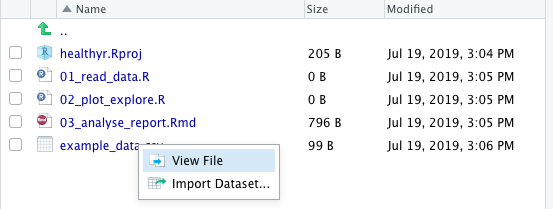
\includegraphics[width=7.68in]{images/chapter02/files_csv_example} \caption{View or import a data file.}\label{fig:chap2-fig-examplecsv}
\end{figure}

Clicking on a data file gives us two options: \texttt{View\ File} or \texttt{Import\ Dataset}.
For standard CSV files, we don't usually bother with the Import interface and just type in (or copy from a previous script):
\index{functions@\textbf{functions}!read\_csv}

\begin{Shaded}
\begin{Highlighting}[]
\KeywordTok{library}\NormalTok{(tidyverse)}
\NormalTok{example_data =}\StringTok{ }\KeywordTok{read_csv}\NormalTok{(}\StringTok{"example_data.csv"}\NormalTok{)}
\end{Highlighting}
\end{Shaded}

Without further arguments, \texttt{read\_csv()} defaults to:

\begin{itemize}
\tightlist
\item
  values are delimited by commas (e.g., \texttt{id,\ var1,\ var2,\ ...});
\item
  numbers use decimal point (e.g., \texttt{4.12}), rather than decimal comma (e.g., \texttt{4,12});
\item
  the first line has column names (it is a ``header'');
\item
  and missing values are empty or denoted NA.
\end{itemize}

If your file, however, is different to these, then the \texttt{Import\ Dataset} interface (Figure \ref{fig:chap2-fig-examplecsv}) is very useful and will give you the relevant \texttt{read\_()} syntax with extra arguments completed for you.

\begin{figure}
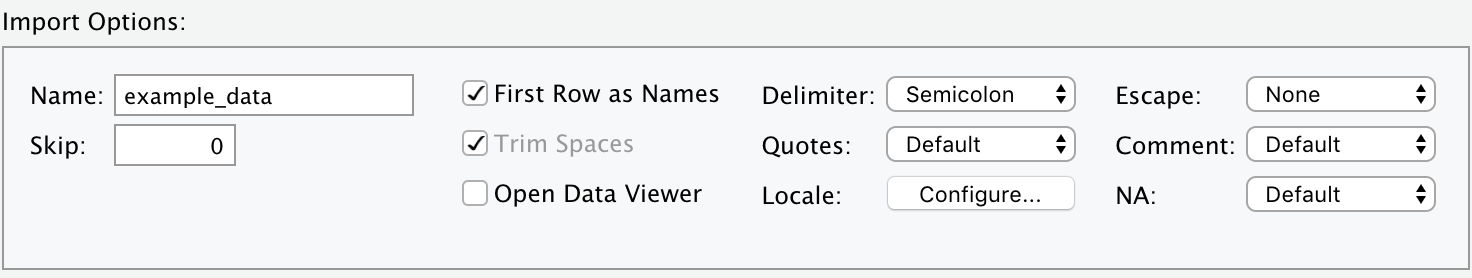
\includegraphics[width=20.44in]{images/chapter02/import_options} \caption{Import: Some of the special settings your data file might have.}\label{fig:chap02-fig-import-tool}
\end{figure}

\begin{figure}
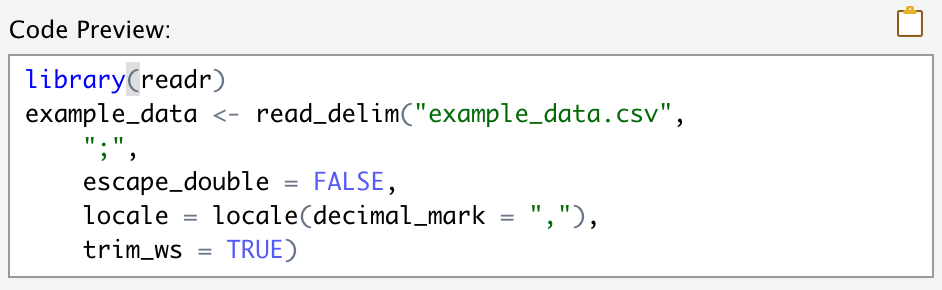
\includegraphics[width=13.08in]{images/chapter02/code_preview} \caption{After using the Import Dataset window, copy-paste the resulting code into your script.}\label{fig:chap02-fig-import-code}
\end{figure}

After selecting the specific options to import file, a friendly preview window will show whether R understands the format of the your data.
DO NOT BE tempted to press the \texttt{Import} button.

Yes, this will read in your dataset once, but means you have to reselect the options every time you come back to RStudio.
Instead, copy-paste the code (e.g., Figure \ref{fig:chap02-fig-import-code}) into your R script - this way you can use it over and over again.

Ensuring all steps are recorded in scripts make your workflow reproducible by your future self, colleagues, supervisors, and extraterrestrials.

\begin{quote}
The \texttt{Import\ Dataset} button can also help you to read in Excel, SPSS, Stata, or SAS files (instead of \texttt{read\_csv()}, it will give you \texttt{read\_excel()}, \texttt{read\_sav()}, \texttt{read\_stata()}, or \texttt{read\_sas()}).
\end{quote}

If you've used R before or are using older scripts passed by colleagues, you might see \texttt{read.csv()} rather than \texttt{read\_csv()}.

In short, \texttt{read\_csv()} is faster and more predictable and in all new scripts this is what you should use.
In existing scripts that work and are tested, do not just start replacing \texttt{read.csv()} with \texttt{read\_csv()}.
\texttt{read\_csv()} handles categorical variables differently \footnote{It does not silently convert strings to factors, i.e., it defaults to \texttt{stringsAsFactors\ =\ FALSE}. For those not familiar with the terminology here - don't worry, we will cover this in just a few sections.}.
An R script written using the \texttt{read.csv()} might not work as expected any more if just replaced with \texttt{read\_csv()}.

\begin{quote}
Do not start updating and possibly breaking existing R scripts by replacing base R functions with the tidyverse ones we show here. Do use the modern functions in any new code you write.
\end{quote}

\hypertarget{reading-in-the-global-burden-of-disease-example-dataset-short-version}{%
\subsection{Reading in the Global Burden of Disease example dataset (short version)}\label{reading-in-the-global-burden-of-disease-example-dataset-short-version}}

In the next few chapters of this book, we will be using the Global Burden of Disease datasets.
The Global Burden of Disease Study (GBD) is the most comprehensive worldwide observational epidemiological study to date.
It describes mortality and morbidity from major diseases, injuries and risk factors to health at global, national and regional levels.
\footnote{Global Burden of Disease Collaborative Network.
  Global Burden of Disease Study 2017 (GBD 2017) Results.
  Seattle, United States: Institute for Health Metrics and Evaluation (IHME), 2018.
  Available from \url{http://ghdx.healthdata.org/gbd-results-tool}.}

GBD data are publicly available from the website.
Table \ref{tab:chap2-tab-gbd} and Figure \ref{fig:chap2-fig-gbd} show a high level version of the project data with just 3 variables: \texttt{cause}, \texttt{year}, \texttt{deaths\_millions} (number of people who die of each cause every year). Later, we will be using a longer dataset with different subgroups and we will show you how to summarise comprehensive datasets yourself.

\begin{Shaded}
\begin{Highlighting}[]
\KeywordTok{library}\NormalTok{(tidyverse)}
\NormalTok{gbd_short =}\StringTok{ }\KeywordTok{read_csv}\NormalTok{(}\StringTok{"data/global_burden_disease_cause-year.csv"}\NormalTok{)}
\end{Highlighting}
\end{Shaded}

\begin{table}[!h]

\caption{\label{tab:chap2-tab-gbd}Deaths per year from three broad disease categories (short version of the Global Burden of Disease example dataset).}
\centering
\fontsize{10}{12}\selectfont
\begin{tabular}[t]{lcr}
\toprule
year & cause & deaths\_millions\\
\midrule
1990 & Communicable diseases & 15.36\\
1990 & Injuries & 4.25\\
1990 & Non-communicable diseases & 26.71\\
\addlinespace
1995 & Communicable diseases & 15.11\\
1995 & Injuries & 4.53\\
1995 & Non-communicable diseases & 29.27\\
\addlinespace
2000 & Communicable diseases & 14.81\\
2000 & Injuries & 4.56\\
2000 & Non-communicable diseases & 31.01\\
\addlinespace
2005 & Communicable diseases & 13.89\\
2005 & Injuries & 4.49\\
2005 & Non-communicable diseases & 32.87\\
\addlinespace
2010 & Communicable diseases & 12.51\\
2010 & Injuries & 4.69\\
2010 & Non-communicable diseases & 35.43\\
\addlinespace
2015 & Communicable diseases & 10.88\\
2015 & Injuries & 4.46\\
2015 & Non-communicable diseases & 39.28\\
\addlinespace
2017 & Communicable diseases & 10.38\\
2017 & Injuries & 4.47\\
2017 & Non-communicable diseases & 40.89\\
\bottomrule
\end{tabular}
\end{table}

\begin{figure}
\centering
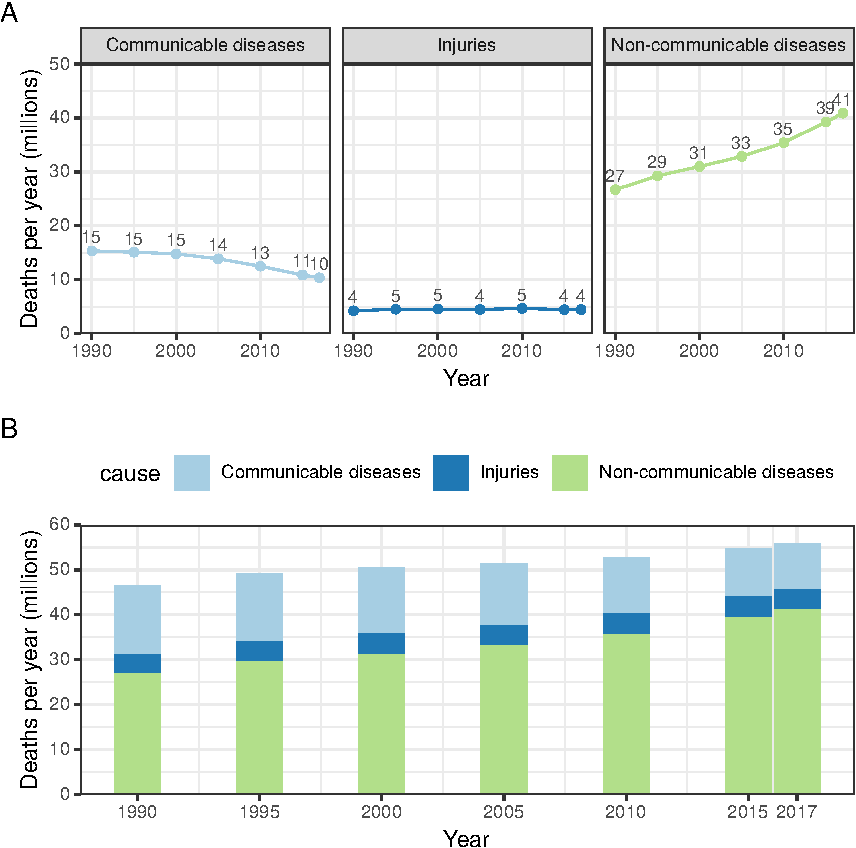
\includegraphics{02_basics_files/figure-latex/chap2-fig-gbd-1.pdf}
\caption{\label{fig:chap2-fig-gbd}Causes of death from the Global Burden of Disease dataset (Table \ref{tab:chap2-tab-gbd}). Data on (B) is the same as (A) but stacked to show the total (sum) of all causes.}
\end{figure}

\hypertarget{variable-types-and-why-we-care}{%
\section{Variable types and why we care}\label{variable-types-and-why-we-care}}

\index{variable types@\textbf{variable types}}
\index{continuous data@\textbf{continuous data}!variable types}
\index{categorical data@\textbf{categorical data}!variable types}
\index{date-time@\textbf{date-time}}

There are three broad types of data:

\begin{itemize}
\tightlist
\item
  continuous (numbers), in R: numeric, double, or integer;
\item
  categorical, in R: character, factor, or logical (TRUE/FALSE);
\item
  date/time, in R: POSIXct date-time\footnote{Portable Operating System Interface (POSIX) is a set of computing standards. There's nothing more to understand about this other than when R starts shouting ``POSIXct this or POSIXlt that'' at you, check your date and time variables}.
\end{itemize}

Values within a column all have to be the same type, but a tibble can of course hold columns of different types.
Generally, R is very good at figuring out what type of data you have (in programming, this `figuring out' is called `parsing').

For example, when reading in data, it will tell you what it assumed for the columns:

\begin{Shaded}
\begin{Highlighting}[]
\KeywordTok{library}\NormalTok{(tidyverse)}
\NormalTok{typesdata =}\StringTok{ }\KeywordTok{read_csv}\NormalTok{(}\StringTok{"data/typesdata.csv"}\NormalTok{)}
\end{Highlighting}
\end{Shaded}

\begin{verbatim}
## Parsed with column specification:
## cols(
##   id = col_character(),
##   group = col_character(),
##   measurement = col_double(),
##   date = col_datetime(format = "")
## )
\end{verbatim}

\begin{Shaded}
\begin{Highlighting}[]
\NormalTok{typesdata}
\end{Highlighting}
\end{Shaded}

\begin{verbatim}
## # A tibble: 3 x 4
##   id    group     measurement date               
##   <chr> <chr>           <dbl> <dttm>             
## 1 ID1   Control           1.8 2017-01-02 12:00:00
## 2 ID2   Treatment         4.5 2018-02-03 13:00:00
## 3 ID3   Treatment         3.7 2019-03-04 14:00:00
\end{verbatim}

This means that a lot of the time you do not have to worry about those little \texttt{\textless{}chr\textgreater{}} vs \texttt{\textless{}dbl\textgreater{}} vs \texttt{\textless{}S3:\ POSIXct\textgreater{}} labels, R knows what its doing.
But in cases of irregular or faulty input data, or when doing a lot of calculations and modifications your data, we need to be aware of these different types to be able to find and fix mistakes.

For example, consider a very similar file as above but with a couple of data entry issues:

\begin{Shaded}
\begin{Highlighting}[]
\NormalTok{typesdata_faulty =}\StringTok{ }\KeywordTok{read_csv}\NormalTok{(}\StringTok{"data/typesdata_faulty.csv"}\NormalTok{)}
\end{Highlighting}
\end{Shaded}

\begin{verbatim}
## Parsed with column specification:
## cols(
##   id = col_character(),
##   group = col_character(),
##   measurement = col_character(),
##   date = col_character()
## )
\end{verbatim}

\begin{Shaded}
\begin{Highlighting}[]
\NormalTok{typesdata_faulty}
\end{Highlighting}
\end{Shaded}

\begin{verbatim}
## # A tibble: 3 x 4
##   id    group     measurement date           
##   <chr> <chr>     <chr>       <chr>          
## 1 ID1   Control   1.8         02-Jan-17 12:00
## 2 ID2   Treatment 4.5         03-Feb-18 13:00
## 3 ID3   Treatment 3.7 or 3.8  04-Mar-19 14:00
\end{verbatim}

Notice R parsed both measurement and date as characters.
The first one is a data entry issue: the person taking the measurement couldn't decide which value to note down (maybe the scale was shifting between the two values) so they included both values and text ``or'' in the cell.

A numeric variable will also get parsed as a categorical variable if it contains certain typos, e.g., if entered as ``3..7'' instead of ``3.7''.

The reason R didn't automatically make sense of the date column is that it can't tell which is the date and which is the year: \textbf{02-Jan-17} could stand for \emph{02-Jan-2017} as well as \emph{2002-Jan-17}.

Therefore, while a lot of the time you do not have to worry about variable types and can just get on with your analysis, it is important to understand what the different types are to be ready to deal with them when issues arise.

\begin{quote}
Since health datasets are generally full of categorical data, it is crucial to understand the difference between characters and factors (both are types of categorical variables in R with pros and cons).
\end{quote}

So here we go.

\hypertarget{numeric-variables-continuous}{%
\section{Numeric variables (continuous)}\label{numeric-variables-continuous}}

\index{variable types@\textbf{variable types}!continuous / numeric}

Number are straightforward to handle and don't usually cause trouble.
R usually refers to numbers as \texttt{numeric} (or \texttt{num}), but sometimes it really gets its nerd on and also calls numbers \texttt{integer} or \texttt{double}.
Integers are numbers without decimal places (e.g., \texttt{1,\ 2,\ 3}), whereas \texttt{double} stands for ``Double-precision floating-point'' format (e.g., \texttt{1.234,\ 5.67890}).

It doesn't usually matter whether R is classifying your continuous data \texttt{numeric/num/double/int}, but it is good to be aware of these different terms as you will see them in R messages.

\begin{quote}
FRIENDLY WARNING: What's about to follow is a bit dry. Furthermore, it is not essential for complete beginners - you might want to continue reading from \textbf{Characters variables}.
Before you leave, take a mental note that sometimes numbers in R have more decimal places than it seems, and that can cause funny behaviour when using the double equals operator (\texttt{==}).
\end{quote}

Something to note about numbers is that R doesn't usually print more than 6 decimal places, but that doesn't mean they don't exist.
For example, from the \texttt{typedata} tibble, we're taking the \texttt{measurement} column and sending it to the \texttt{mean()} function.
R then calculates the mean and tells us what it is with 6 decimal places:

\begin{Shaded}
\begin{Highlighting}[]
\NormalTok{typesdata}\OperatorTok{$}\NormalTok{measurement }\OperatorTok\StringTok{ }\KeywordTok{mean}\NormalTok{()}
\end{Highlighting}
\end{Shaded}

\begin{verbatim}
## [1] 3.333333
\end{verbatim}

Let' save that in a new object:

\begin{Shaded}
\begin{Highlighting}[]
\NormalTok{measurement_mean =}\StringTok{ }\NormalTok{typesdata}\OperatorTok{$}\NormalTok{measurement }\OperatorTok\StringTok{ }\KeywordTok{mean}\NormalTok{()}
\end{Highlighting}
\end{Shaded}

But when using the double equals operator to check if this is equivalent to a fixed value (you might do this when comparing to a threshold, or even another mean value), R returns \texttt{FALSE}:

\begin{Shaded}
\begin{Highlighting}[]
\NormalTok{measurement_mean }\OperatorTok{==}\StringTok{ }\FloatTok{3.333333}
\end{Highlighting}
\end{Shaded}

\begin{verbatim}
## [1] FALSE
\end{verbatim}

Now this doesn't seem right, does it - R clearly told us just above that the mean of this variable is 3.333333 (reminder: the actual values in the measurement column are 1.8, 4.5, 3.7).
The reason the above statement is \texttt{FALSE} is because \texttt{measurement\_mean} is quietly holding more than 6 decimal places.

One way to go about this is to round the mean to a reasonable number of decimal places:

\index{functions@\textbf{functions}!round}

\begin{Shaded}
\begin{Highlighting}[]
\KeywordTok{round}\NormalTok{(measurement_mean, }\DecValTok{3}\NormalTok{)}
\end{Highlighting}
\end{Shaded}

\begin{verbatim}
## [1] 3.333
\end{verbatim}

The second argument of \texttt{round()} specifies the number of decimal places you want your number(s) rounded to.
So when using \texttt{round()} in the equality statement like this, we get the expected \texttt{TRUE}:

\begin{Shaded}
\begin{Highlighting}[]
\KeywordTok{round}\NormalTok{(measurement_mean, }\DecValTok{3}\NormalTok{) }\OperatorTok{==}\StringTok{ }\FloatTok{3.333}
\end{Highlighting}
\end{Shaded}

\begin{verbatim}
## [1] TRUE
\end{verbatim}

Which is usually fine, especially if you've finished applying calculations on that number.
But when you indent to use it if further calculations, then rounding should be left to the very end - to minimise rounding errors.
This is where the \texttt{near()} function comes in handy:

\index{functions@\textbf{functions}!near}

\begin{Shaded}
\begin{Highlighting}[]
\KeywordTok{library}\NormalTok{(tidyverse)}
\KeywordTok{near}\NormalTok{(measurement_mean, }\FloatTok{3.333}\NormalTok{, }\FloatTok{0.001}\NormalTok{)}
\end{Highlighting}
\end{Shaded}

\begin{verbatim}
## [1] TRUE
\end{verbatim}

The first two arguments for \texttt{near()} are the numbers you are comparing, the third argument is the precision you are interested in. So if the numbers are equal within that precision, it returns \texttt{TRUE}.
This means you get the expected result without having to round the numbers off.

\hypertarget{character-variables}{%
\section{Character variables}\label{character-variables}}

\index{variable types@\textbf{variable types}!character}

\textbf{Characters} (sometimes referred to as \emph{strings} or \emph{character strings}) in R are letters, words, or even whole sentences (an example of this may be free text comments).
Characters are displayed in-between \texttt{""} (or \texttt{\textquotesingle{}\textquotesingle{}}).

A very useful function for quickly investigating categorical variables is the \texttt{count()} function:

\begin{Shaded}
\begin{Highlighting}[]
\KeywordTok{library}\NormalTok{(tidyverse)}
\NormalTok{typesdata }\OperatorTok
\StringTok{  }\KeywordTok{count}\NormalTok{(group)}
\end{Highlighting}
\end{Shaded}

\begin{verbatim}
## # A tibble: 2 x 2
##   group         n
##   <chr>     <int>
## 1 Control       1
## 2 Treatment     2
\end{verbatim}

\texttt{count()} can accept multiple variables and will count up the number of observations in each subgroup, e.g., \texttt{mydata\ \%\textgreater{}\%\ count(var1,\ var2)}.

Another helpful option to count is \texttt{sort\ =\ TRUE}, which will order the result putting the highest count (\texttt{n}) to the top.

\begin{Shaded}
\begin{Highlighting}[]
\NormalTok{typesdata }\OperatorTok
\StringTok{  }\KeywordTok{count}\NormalTok{(group, }\DataTypeTok{sort =} \OtherTok{TRUE}\NormalTok{)}
\end{Highlighting}
\end{Shaded}

\begin{verbatim}
## # A tibble: 2 x 2
##   group         n
##   <chr>     <int>
## 1 Treatment     2
## 2 Control       1
\end{verbatim}

\texttt{count()}with the \texttt{sort\ =\ TRUE} option is also useful for identifying duplicate IDs or misspellings in your data.
With this example \texttt{tibble} (\texttt{typesdata}) that only has three rows, it is easy to see that the \texttt{id} column is a unique identifier whereas the \texttt{group} column is a categorical variable.

You can check everything by just eyeballing the \texttt{tibble} using the built in Viewer tab (click on the dataset in the Environment tab).

But for larger datasets, you need to know how to check and then clean data programmatically - you can't go through thousands of values checking they are all as intended without unexpected duplicates or typos.

For most variables (categorical or numeric) we recommend always plotting your data before starting analysis.
But to check for duplicates in a unique identifier, use \texttt{count()} with \texttt{sort\ =\ TRUE}:

\begin{Shaded}
\begin{Highlighting}[]
\CommentTok{# all ids are unique:}
\NormalTok{typesdata }\OperatorTok\StringTok{ }
\StringTok{  }\KeywordTok{count}\NormalTok{(id, }\DataTypeTok{sort =} \OtherTok{TRUE}\NormalTok{)}
\end{Highlighting}
\end{Shaded}

\begin{verbatim}
## # A tibble: 3 x 2
##   id        n
##   <chr> <int>
## 1 ID1       1
## 2 ID2       1
## 3 ID3       1
\end{verbatim}

\begin{Shaded}
\begin{Highlighting}[]
\CommentTok{# we add in a duplicate row where id = ID3,}
\CommentTok{# then count again:}
\NormalTok{typesdata }\OperatorTok\StringTok{ }
\StringTok{  }\KeywordTok{add_row}\NormalTok{(}\DataTypeTok{id =} \StringTok{"ID3"}\NormalTok{) }\OperatorTok\StringTok{ }
\StringTok{  }\KeywordTok{count}\NormalTok{(id, }\DataTypeTok{sort =} \OtherTok{TRUE}\NormalTok{)}
\end{Highlighting}
\end{Shaded}

\begin{verbatim}
## # A tibble: 3 x 2
##   id        n
##   <chr> <int>
## 1 ID3       2
## 2 ID1       1
## 3 ID2       1
\end{verbatim}

\hypertarget{factor-variables-categorical}{%
\section{Factor variables (categorical)}\label{factor-variables-categorical}}

\index{variable types@\textbf{variable types}!categorical / factor}

\textbf{Factors} are fussy characters.
Factors are fussy because they have something called \textbf{levels}.
Levels are all the unique values a factor variable could take, e.g.~like when we looked at \texttt{typesdata\$group\ \%\textgreater{}\%\ unique()}.
Using factors rather than just characters can be useful because:

\begin{itemize}
\tightlist
\item
  The values factor levels can take is fixed.
  For example, once you tell R that \texttt{typesdata\$group} is a factor with two levels: Control and Treatment, combining it with other datasets with different spellings or abbreviations for the same variable will generate a warning.
  This can be helpful but can also be a nuisance when you really do want to add in another level to a \texttt{factor} variable.
\item
  Levels have an order.
  When running statistical tests on grouped data (e.g., Control vs Treatment, Adult vs Child) and the variable is just a character, not a factor, R will use the alphabetically first as the reference level.
  Converting a character column into a factor column enables us to define and change the order of its levels.
  Level order affects many things including regression results and plots: by default, categorical variables are ordered alphabetically.
  If we want a different order in say a bar plot, we need to convert to a factor and reorder before we plot it.
  The plot will then know how the order it better.
\end{itemize}

So overall, since health data is often categorical and has a reference (comparison) level, then factors are an essential way to work with these data in R.
Nevertheless, the fussiness of factors can sometimes be unhelpful or even frustrating.
A lot more about factor handling will be covered later in the book.

\hypertarget{datetime-variables}{%
\section{Date/time variables}\label{datetime-variables}}

\index{variable types@\textbf{variable types}!date-time}
\index{functions@\textbf{functions}!dmy}
\index{functions@\textbf{functions}!ymd}

R is very good for working with dates.
For example, it can calculate the number of days/weeks/months between two dates, or it can be used to find a future date is (e.g., ``what's the date exactly 60 days from now?'').
It also knows about time zones and is happy to parse dates in pretty much any format - as long as you tell R how your date is formatted (e.g., day before month, month name abbreviated, year in 2 or 4 digits, etc.).
Since R displays dates and times between quotes (""), they look similar to characters. However, it is important to know whether R has understood which of your columns contain date/time information, as which are just normal characters.

\begin{Shaded}
\begin{Highlighting}[]
\KeywordTok{library}\NormalTok{(lubridate) }\CommentTok{# lubridate makes working with dates easier}
\NormalTok{current_datetime =}\StringTok{ }\KeywordTok{Sys.time}\NormalTok{()}
\NormalTok{current_datetime}
\end{Highlighting}
\end{Shaded}

\begin{verbatim}
## [1] "2020-01-27 06:45:23 PST"
\end{verbatim}

\begin{Shaded}
\begin{Highlighting}[]
\NormalTok{my_datetime =}\StringTok{ "2020-12-01 12:00"}
\NormalTok{my_datetime}
\end{Highlighting}
\end{Shaded}

\begin{verbatim}
## [1] "2020-12-01 12:00"
\end{verbatim}

When printed, the two objects - \texttt{current\_datetime} and \texttt{my\_datetime} seem to have the a very similar format.
But if we try to calculate the difference between these two dates, we get an error:

\begin{Shaded}
\begin{Highlighting}[]
\NormalTok{my_datetime }\OperatorTok{-}\StringTok{ }\NormalTok{current_datetime}
\end{Highlighting}
\end{Shaded}

\begin{verbatim}
## Error in `-.POSIXt`(my_datetime, current_datetime): can only subtract from "POSIXt" objects
\end{verbatim}

That's because when we assigned a value to \texttt{my\_datetime}, R assumed the simpler type for it - so a character.
We can check what the type of an object or variable is using the \texttt{class()} function:

\begin{Shaded}
\begin{Highlighting}[]
\NormalTok{current_datetime }\OperatorTok\StringTok{ }\KeywordTok{class}\NormalTok{()}
\end{Highlighting}
\end{Shaded}

\begin{verbatim}
## [1] "POSIXct" "POSIXt"
\end{verbatim}

\begin{Shaded}
\begin{Highlighting}[]
\NormalTok{my_datetime }\OperatorTok\StringTok{ }\KeywordTok{class}\NormalTok{()}
\end{Highlighting}
\end{Shaded}

\begin{verbatim}
## [1] "character"
\end{verbatim}

So we need to tell R that \texttt{my\_datetime} does indeed include date/time information so we can then use it in calculations:

\begin{Shaded}
\begin{Highlighting}[]
\NormalTok{my_datetime_converted =}\StringTok{ }\KeywordTok{ymd_hm}\NormalTok{(my_datetime)}
\NormalTok{my_datetime_converted}
\end{Highlighting}
\end{Shaded}

\begin{verbatim}
## [1] "2020-12-01 12:00:00 UTC"
\end{verbatim}

Calculating the difference will now work:

\begin{Shaded}
\begin{Highlighting}[]
\NormalTok{my_datetime_converted }\OperatorTok{-}\StringTok{ }\NormalTok{current_datetime}
\end{Highlighting}
\end{Shaded}

\begin{verbatim}
## Time difference of 308.8851 days
\end{verbatim}

Since R knows this is a difference between two date/time objects, it prints the in a nicely readable way.
Furthermore, the result has its own type, it is a ``difftime''.

\begin{Shaded}
\begin{Highlighting}[]
\NormalTok{my_datesdiff =}\StringTok{ }\NormalTok{my_datetime_converted }\OperatorTok{-}\StringTok{ }\NormalTok{current_datetime}
\NormalTok{my_datesdiff }\OperatorTok\StringTok{ }\KeywordTok{class}\NormalTok{()}
\end{Highlighting}
\end{Shaded}

\begin{verbatim}
## [1] "difftime"
\end{verbatim}

This is useful if we want to apply this time difference on another date, e.g.:

\begin{Shaded}
\begin{Highlighting}[]
\KeywordTok{ymd_hm}\NormalTok{(}\StringTok{"2021-01-02 12:00"}\NormalTok{) }\OperatorTok{+}\StringTok{ }\NormalTok{my_datesdiff}
\end{Highlighting}
\end{Shaded}

\begin{verbatim}
## [1] "2021-11-07 09:14:36 UTC"
\end{verbatim}

But if we want to use the number of days in a normal calculation, e.g., what if a measurement increased by 560 arbitrary units during this time period.
We might want to calculate the increase per day like this:

\begin{Shaded}
\begin{Highlighting}[]
\DecValTok{560}\OperatorTok{/}\NormalTok{my_datesdiff}
\end{Highlighting}
\end{Shaded}

\begin{verbatim}
## Error in `/.difftime`(560, my_datesdiff): second argument of / cannot be a "difftime" object
\end{verbatim}

Doesn't work, does it.
We need to convert \texttt{my\_datesdiff} (which is a difftime value) into a numeric value by using the \texttt{as.numeric()} function:

\begin{Shaded}
\begin{Highlighting}[]
\DecValTok{560}\OperatorTok{/}\KeywordTok{as.numeric}\NormalTok{(my_datesdiff)}
\end{Highlighting}
\end{Shaded}

\begin{verbatim}
## [1] 1.812972
\end{verbatim}

The lubridate package comes with several convenient functions for parsing dates, e.g., \texttt{ymd()}, \texttt{mdy()}, \texttt{ymd\_hm()}, etc. - for a full list see lubridate.tidyverse.org.

However, if your date/time variable comes in an extra special format, then use the \texttt{parse\_date\_time()} function where the second argument specifies the format using these helpers:

\begin{longtable}[]{@{}lll@{}}
\toprule
Notation & Meaning & Example\tabularnewline
\midrule
\endhead
\texttt{\%d} & day as number & 01-31\tabularnewline
\texttt{\%m} & month as number & 01-12\tabularnewline
\texttt{\%B} & month name & January-December\tabularnewline
\texttt{\%b} & abbreviated month & Jan-Dec\tabularnewline
\texttt{\%Y} & 4-digit year & 2019\tabularnewline
\texttt{\%y} & 2-digit year & 19\tabularnewline
\texttt{\%H} & hours & 12\tabularnewline
\texttt{\%M} & minutes & 01\tabularnewline
\texttt{\%A} & weekday & Monday-Sunday\tabularnewline
\texttt{\%a} & abbreviated weekday & Mon-Sun\tabularnewline
\bottomrule
\end{longtable}

For example:

\begin{Shaded}
\begin{Highlighting}[]
\KeywordTok{parse_date_time}\NormalTok{(}\StringTok{"12:34 07/Jan'20"}\NormalTok{, }\StringTok{"%H:%M %d/%b'%y"}\NormalTok{)}
\end{Highlighting}
\end{Shaded}

\begin{verbatim}
## [1] "2020-01-07 12:34:00 UTC"
\end{verbatim}

Furthermore, the same date/time helpers can be used to rearrange your date and time for printing:

\begin{Shaded}
\begin{Highlighting}[]
\KeywordTok{Sys.time}\NormalTok{()}
\end{Highlighting}
\end{Shaded}

\begin{verbatim}
## [1] "2020-01-27 06:45:23 PST"
\end{verbatim}

\begin{Shaded}
\begin{Highlighting}[]
\KeywordTok{Sys.time}\NormalTok{() }\OperatorTok\StringTok{ }\KeywordTok{format}\NormalTok{(}\StringTok{"%H:%M on %B-%d (%Y)"}\NormalTok{)}
\end{Highlighting}
\end{Shaded}

\begin{verbatim}
## [1] "06:45 on January-27 (2020)"
\end{verbatim}

You can even add plain text into the \texttt{format()} function, R will know to put the right date/time values where the \texttt{\%} are:

\begin{Shaded}
\begin{Highlighting}[]
\KeywordTok{Sys.time}\NormalTok{() }\OperatorTok\StringTok{ }\KeywordTok{format}\NormalTok{(}\StringTok{"Happy days, the current time is %H:%M %B-%d (%Y)!"}\NormalTok{)}
\end{Highlighting}
\end{Shaded}

\begin{verbatim}
## [1] "Happy days, the current time is 06:45 January-27 (2020)!"
\end{verbatim}

\hypertarget{objects-and-functions}{%
\section{Objects and functions}\label{objects-and-functions}}

\index{objects}
\index{functions@\textbf{functions}}

There are two fundamental concepts in statistical programming that it is important to get straight from the outset - objects and functions.
As throughout this book, we will introduce new concepts using specific examples first.

The most common data object you will be working with is a table.
This is something with rows and columns much like the example in Table \ref{tab:chap2-tab-examp1}.

\begin{table}

\caption{\label{tab:chap2-tab-examp1}Example of a table including missing values denoted NA (Not applicable/Not available).}
\centering
\fontsize{8}{10}\selectfont
\begin{tabular}[t]{rlrrr}
\toprule
id & sex & var1 & var2 & var3\\
\midrule
1 & Male & 4 & NA & 2\\
2 & Female & 1 & 4 & 1\\
3 & Female & 2 & 5 & NA\\
4 & Male & 3 & NA & NA\\
\bottomrule
\end{tabular}
\end{table}

A table can live anywhere: on paper, in a Spreadsheet, in an SQL database, or it can live in your R Session's Environment.
And yes, R sessions are as fun as they sound, almost as fun as music sessions.

We usually initiate and interface R using RStudio, but everything we talk about here (objects, functions, sessions, environment) also work when RStudio is not available, but R is.
This can be the case if you are working on a supercomputer that can only serve the R Console, and not an RStudio IDE (reminder from first chapter: Integrated Development Environment).

So, regularly shaped data in rows and columns is called a table when it lives outside R, but once you read it into R (import it), we call it a tibble.
\footnote{There is also the original version of tables in R - they are called data frames.
  In most cases, \texttt{data\ frames} and \texttt{tibbles} work interchangeably, but \texttt{tibbles} often work better.
  Another great alternative to base R \texttt{data\ frames} are \texttt{data\ tables}.
  In this book, and for most of our day-to-day work these days, we will use \texttt{tibbles}.}

When you are in one of your very cool R sessions and read in some data, it goes into this session's Environment.
Everything in your Environment needs to have a name.
You will likely have many objects such as tibbles going on at the same time.
Note that \texttt{tibble} is what the thing is, rather than its name.
This is the \texttt{class} of an object.

To keep our code examples easy to follow, we call our example tibble \texttt{mydata}.
In a real analysis, you should give your tibbles meaningful names, e.g., \texttt{patient\_data}, \texttt{lab\_results}, \texttt{annual\_totals}, etc.

So, the tibble named \texttt{mydata} is example of an object that can be in the Environment of your R Session:

\begin{Shaded}
\begin{Highlighting}[]
\NormalTok{mydata}
\end{Highlighting}
\end{Shaded}

\begin{verbatim}
## # A tibble: 4 x 5
##      id sex     var1  var2  var3
##   <int> <chr>  <dbl> <dbl> <dbl>
## 1     1 Male       4    NA     2
## 2     2 Female     1     4     1
## 3     3 Female     2     5    NA
## 4     4 Male       3    NA    NA
\end{verbatim}

So what is a function?

A function is a procedure which takes some information (input), does something to it, and passes back the modified information (output).

A simple function that can be applied to numeric data for instance is \texttt{mean()}.

R functions always have round brackets after their name.
This is for two reasons.
First, it easily differentiates them as functions - you will get used to reading them like this.\\
Second, and more important, we can put \textbf{arguments} in these brackets.

Arguments can also be thought of as input.
In data analysis, the most common input for a function is data - we need to give \texttt{mean()} some data to average over.
It does not make sense (nor will it work) to feed \texttt{mean()} the whole tibble with multiple columns, including patient IDs and a categorical variable (\texttt{sex}).

To quickly extract a single column, we use the \texttt{\$} symbol like this:
\index{symbols@\textbf{symbols}!select column \texttt{\$}}

\begin{Shaded}
\begin{Highlighting}[]
\NormalTok{mydata}\OperatorTok{$}\NormalTok{var1}
\end{Highlighting}
\end{Shaded}

\begin{verbatim}
## [1] 4 1 2 3
\end{verbatim}

You can ignore the \texttt{\#\#\ {[}1{]}} at the beginning of the extracted values - this is something that becomes more useful when printing multiple lines of data as the number in the square brackets keeps count on how many values we are seeing.

We can then use \texttt{mydata\$var1} as the first argument of \texttt{mean()} by putting it inside its brackets:

\begin{Shaded}
\begin{Highlighting}[]
\KeywordTok{mean}\NormalTok{(mydata}\OperatorTok{$}\NormalTok{var1)}
\end{Highlighting}
\end{Shaded}

\begin{verbatim}
## [1] 2.5
\end{verbatim}

Which tells us that the mean of \texttt{var1} (4, 1, 2, 3) is 2.5.
In this example, \texttt{mydata\$var1} is the first and only argument to \texttt{mean()}.
But what happens if we try to calculate the average value of \texttt{var2} (NA, 4, 5, NA)?

\begin{Shaded}
\begin{Highlighting}[]
\KeywordTok{mean}\NormalTok{(mydata}\OperatorTok{$}\NormalTok{var2)}
\end{Highlighting}
\end{Shaded}

\begin{verbatim}
## [1] NA
\end{verbatim}

We get an \texttt{NA} (``Not applicable'').
We would expect to see an \texttt{NA} if we tried to, for example, calculate the average of \texttt{sex}:

\begin{Shaded}
\begin{Highlighting}[]
\KeywordTok{mean}\NormalTok{(mydata}\OperatorTok{$}\NormalTok{sex)}
\end{Highlighting}
\end{Shaded}

\begin{verbatim}
## Warning in mean.default(mydata$sex): argument is not numeric or logical:
## returning NA
\end{verbatim}

\begin{verbatim}
## [1] NA
\end{verbatim}

In fact, in this case, R also gives us a pretty clear warning suggesting it can't compute the mean of an argument that is not numeric or logical.
The sentence actually reads pretty fun, as if R was saying it was not logical to calculate the mean of something that is not numeric.

But what R is actually saying that it is happy to calculate the mean of two types of variables: numerics or logicals, but what you have passed is neither.
\footnote{Logical is a data type with two potential values: TRUE or FALSE.
  We will come back to data types.}

So why does \texttt{mean(mydata\$var2)} return \texttt{NA} rather than the mean of the numeric values included in this column?
That is because the column itself includes missing values (\texttt{NAs}), and R does not want to average over NAs implicitly.
It is being cautious - what if you didn't know there were missing values for some patients?
If you wanted to compare the means of \texttt{var1} and \texttt{var2} without any further filtering, you would be comparing samples of different sizes.

If you decide to ignore the NAs and want to calculate the mean anyway, you can do so by adding another argument to \texttt{mean()}:

\index{missing values remove \texttt{na.rm}}\}

\begin{Shaded}
\begin{Highlighting}[]
\KeywordTok{mean}\NormalTok{(mydata}\OperatorTok{$}\NormalTok{var2, }\DataTypeTok{na.rm =} \OtherTok{TRUE}\NormalTok{)}
\end{Highlighting}
\end{Shaded}

\begin{verbatim}
## [1] 4.5
\end{verbatim}

Adding \texttt{na.rm\ =\ TRUE} tells R that you are happy for it to calculate the mean of any existing values (but to remove - \texttt{rm} - the \texttt{NA} values).
This `removal' excludes the NAs from the calculation, it does not affect the actual tibble (\texttt{mydata}) holding the dataset.

R is case sensitive, so \texttt{na.rm}, not \texttt{NA.rm} etc.
There is, however, no need to memorize how the arguments of functions are exactly spelled - this is what the Help tab is for (press \texttt{F1} when the cursor is on the name of the function).
Help pages are built into R, so an internet connection is not required for this.

\begin{quote}
Make sure to separate multiple arguments with commas or R will give you an error of \texttt{Error:\ unexpected\ symbol}.
\end{quote}

Finally, some functions do not need any arguments to work.
A good example is the \texttt{Sys.time()} which returns the current time and date.
This is very useful when using R to generate and update reports automatically.
Including this means you can always be clear on when the results were last updated.

\index{functions@\textbf{functions}!Sys.time}
\index{system time}

\begin{Shaded}
\begin{Highlighting}[]
\KeywordTok{Sys.time}\NormalTok{()}
\end{Highlighting}
\end{Shaded}

\begin{verbatim}
## [1] "2020-01-27 06:45:23 PST"
\end{verbatim}

To summarise, objects and functions work hand in hand.
Objects are both an input as well as the output of a function (what the function returns).

When passing data to a functon is is usually its first argument, with further arguments used to specify behaviour.

When we say ``the function returns'', we are referring to its output (or an Error if it's one of those days).

The returned object can be different to its input object.
In our \texttt{mean()} example above, the input object was a column (\texttt{mydata\$var1}: 4, 1, 2, 3), whereas the output was a single value: 2.5.

\hypertarget{working-with-objects}{%
\section{Working with Objects}\label{working-with-objects}}

To create a new object in our Environment we use the equals sign:
\index{symbols@\textbf{symbols}!assignment \texttt{=}}

\begin{Shaded}
\begin{Highlighting}[]
\NormalTok{a =}\StringTok{ }\DecValTok{103}
\end{Highlighting}
\end{Shaded}

This reads: the object \texttt{a} is assigned value 103.
You know that the assignment worked when it shows up in the Environment tab.
If we now run \texttt{a} just on its own, it gets printed back to us:

\begin{Shaded}
\begin{Highlighting}[]
\NormalTok{a}
\end{Highlighting}
\end{Shaded}

\begin{verbatim}
## [1] 103
\end{verbatim}

Similarly, if we run a function without assignment to an object, it gets printed but not saved in your Environment:
\index{functions@\textbf{functions}!seq}

\begin{Shaded}
\begin{Highlighting}[]
\KeywordTok{seq}\NormalTok{(}\DecValTok{15}\NormalTok{, }\DecValTok{30}\NormalTok{)}
\end{Highlighting}
\end{Shaded}

\begin{verbatim}
##  [1] 15 16 17 18 19 20 21 22 23 24 25 26 27 28 29 30
\end{verbatim}

\texttt{seq()} is a function that creates a sequence of numbers (+1 by default) between the two arguments you pass to it in its brackets.
We can assign the result of \texttt{seq(15,\ 30)} into an object, let's call it \texttt{example\_sequence}:

\begin{Shaded}
\begin{Highlighting}[]
\NormalTok{example_sequence =}\StringTok{ }\KeywordTok{seq}\NormalTok{(}\DecValTok{15}\NormalTok{, }\DecValTok{30}\NormalTok{)}
\end{Highlighting}
\end{Shaded}

Doing this creates \texttt{example\_sequence} in our Environment, but it does not print it.

\begin{quote}
If you save the results of an R function in an object, it does not get printed.
If you run a function without the assignment (\texttt{=}), its results get printed, but not saved in an object.
\end{quote}

You can call your object pretty much anything you want, as long as it starts with a letter.
It can then include numbers as well, for example, we could have named the new object \texttt{sequence\_15\_to\_30}.
Spaces in object names are not easy to work with, we tend to use underscores in their place, but you could also use capitalization, e.g. \texttt{exampleSequence\ =\ seq(15,\ 30)}.

Finally, R doesn't mind overwriting an existing object, for example (notice how we then include the variable on a new line to get it printed as well as overwritten):

\begin{Shaded}
\begin{Highlighting}[]
\NormalTok{example_sequence =}\StringTok{ }\NormalTok{example_sequence}\OperatorTok{/}\DecValTok{2}

\NormalTok{example_sequence}
\end{Highlighting}
\end{Shaded}

\begin{verbatim}
##  [1]  7.5  8.0  8.5  9.0  9.5 10.0 10.5 11.0 11.5 12.0 12.5 13.0 13.5 14.0 14.5
## [16] 15.0
\end{verbatim}

\begin{quote}
Note that many people use \texttt{\textless{}-} instead of \texttt{=}.
They mean the same thing in R: both \texttt{=} and \texttt{\textless{}-} save what is on the right into an object with the name on the left.
There is also a left-to-right operator: \texttt{-\textgreater{}}.
\end{quote}

\hypertarget{pipe--}{%
\section{\texorpdfstring{Pipe - \texttt{\%\textgreater{}\%}}{Pipe - \%\textgreater{}\%}}\label{pipe--}}

\index{symbols@\textbf{symbols}!pipe \texttt{\%>\%}}
\index{pipe@\textbf{pipe}}

The pipe - denoted \texttt{\%\textgreater{}\%} - is probably the oddest looking thing you'll see in this book.
But please bear with, it is not as scary as it looks!
Furthermore, it is super useful.
We use the pipe to send objects into functions.

In the above examples, we calculated the mean of column \texttt{var1} from \texttt{mydata} by \texttt{mean(mydata\$var1)}. With the pipe, we can rewrite this as:

\begin{Shaded}
\begin{Highlighting}[]
\KeywordTok{library}\NormalTok{(tidyverse)}
\NormalTok{mydata}\OperatorTok{$}\NormalTok{var1 }\OperatorTok\StringTok{ }\KeywordTok{mean}\NormalTok{()}
\end{Highlighting}
\end{Shaded}

\begin{verbatim}
## [1] 2.5
\end{verbatim}

Which reads: ``Working with \texttt{mydata}, we select a single column called \texttt{var1} (with the \texttt{\$}) \textbf{and then} calculate the \texttt{mean()}.'' The pipe becomes especially useful once the analysis includes multiple steps applied one after another.
A good way to read and think of the pipe is \textbf{``and then''}.

This piping business is not standard R functionality and before using it in a script, you need to tell R this is what you will be doing.
The pipe comes from the \textbf{magrittr} package (Figure \ref{fig:chap2-fig-pipe}), but loading the \textbf{tidyverse} will also load the pipe.
So library(tidyverse) initialises everything you need (no need to include library(magrittr) explicitly).

\begin{quote}
To insert a pipe \texttt{\%\textgreater{}\%}, use the keyboard shortcut \texttt{Ctrl+Shift+M}.
\end{quote}

With or without the pipe, the general rule ``if the result gets printed it doesn't get saved'' still applies.
To save the result of the function into a new object (so it shows up in the Environment), you need to add the name of the new object with the assignment operator (\texttt{=}):

\begin{Shaded}
\begin{Highlighting}[]
\NormalTok{mean_result =}\StringTok{ }\NormalTok{mydata}\OperatorTok{$}\NormalTok{var1 }\OperatorTok\StringTok{ }\KeywordTok{mean}\NormalTok{()}
\end{Highlighting}
\end{Shaded}

\textbackslash{}begin\{figure\}

\includegraphics[width=5.56in]{images/chapter02/magrittr} \textbackslash{}caption\{This is not a pipe. René Magritte inspired artwork by Stefan Milton Bache (creator of \texttt{\%\textgreater{}\%} in R). Image source: \url{https://cran.r-project.org/web/packages/magrittr/vignettes/magrittr.html}\}\label{fig:chap2-fig-pipe}
\textbackslash{}end\{figure\}

\hypertarget{when-pipe-sends-data-to-the-wrong-place-use-.-to-direct-it}{%
\subsection{When pipe sends data to the wrong place: use . to direct it}\label{when-pipe-sends-data-to-the-wrong-place-use-.-to-direct-it}}

The pipe usually sends data to the beginning of function brackets (as most of the functions we use expect a tibble as the first argument).
So \texttt{mydata\ \%\textgreater{}\%\ lm(dependent\textasciitilde{}explanatory)} is equivalent to \texttt{lm(mydata,\ dependent\textasciitilde{}explanatory)}. \texttt{lm()} - linear model - will be introduced in detail in Chapter \ref{chap07-h1}.

However, the \texttt{lm()} function does not expect data as its first argument.
\texttt{lm()} wants us to specify the variables first (\texttt{dependent\textasciitilde{}explanatory}), and then wants the tibble these columns are in.
So we have to use the \texttt{.} to tell the pipe to send the data to the second argument of \texttt{lm()}, not the first, e.g.

\begin{Shaded}
\begin{Highlighting}[]
\NormalTok{mydata }\OperatorTok\StringTok{ }
\StringTok{  }\KeywordTok{lm}\NormalTok{(var1}\OperatorTok{~}\NormalTok{var2, }\DataTypeTok{data =}\NormalTok{ .)}
\end{Highlighting}
\end{Shaded}

\hypertarget{operators-for-filtering-data}{%
\section{Operators for filtering data}\label{operators-for-filtering-data}}

\index{operators}
\index{functions@\textbf{functions}!filter}
\index{symbols@\textbf{symbols}!less than \texttt{<}}
\index{symbols@\textbf{symbols}!greater than \texttt{>}}
\index{symbols@\textbf{symbols}!less or equal \texttt{<=}}
\index{symbols@\textbf{symbols}!greater or equal \texttt{>=}}
\index{symbols@\textbf{symbols}!equal \texttt{=}}
\index{symbols@\textbf{symbols}!not \texttt{"!}}
\index{symbols@\textbf{symbols}!AND \texttt{\&}}
\index{symbols@\textbf{symbols}!OR \texttt{"|}}

Operators are symbols that tell R how to handle different pieces of data or objects.
We have already introduced three: \texttt{\$} (selects a column), \texttt{=} (assigns values or results to a variable), and the pipe - \texttt{\%\textgreater{}\%} (sends data into a function).

Other common operators are the ones we use for filtering data - these are called comparison and logical operators.
This may be for creating subgroups, or for excluding outliers or incomplete cases.

The comparison operators that work with numeric data are relatively straightforward: \texttt{\textgreater{},\ \textless{},\ \textgreater{}=,\ \textless{}=}.
The first two check whether your values are greater or less than another value, the last two check for ``greater than or equal to'' and "less than or equal to. These operators are most commonly spotted inside the \texttt{filter()} function:

\begin{Shaded}
\begin{Highlighting}[]
\NormalTok{gbd_short }\OperatorTok\StringTok{ }
\StringTok{  }\KeywordTok{filter}\NormalTok{(year }\OperatorTok{<}\StringTok{ }\DecValTok{1995}\NormalTok{)}
\end{Highlighting}
\end{Shaded}

\begin{verbatim}
## # A tibble: 3 x 3
##    year cause                     deaths_millions
##   <dbl> <chr>                               <dbl>
## 1  1990 Communicable diseases               15.4 
## 2  1990 Injuries                             4.25
## 3  1990 Non-communicable diseases           26.7
\end{verbatim}

Here we send the data (\texttt{gbd\_short}) to the \texttt{filter()} and ask it to retain all years that are less than 1995.
The resulting tibble only includes the year 1990.
Now, if we use the \texttt{\textless{}=} (less than or equal to) operator, both 1990 and 1995 pass the filter:

\begin{Shaded}
\begin{Highlighting}[]
\NormalTok{gbd_short }\OperatorTok\StringTok{ }
\StringTok{  }\KeywordTok{filter}\NormalTok{(year }\OperatorTok{<=}\StringTok{ }\DecValTok{1995}\NormalTok{)}
\end{Highlighting}
\end{Shaded}

\begin{verbatim}
## # A tibble: 6 x 3
##    year cause                     deaths_millions
##   <dbl> <chr>                               <dbl>
## 1  1990 Communicable diseases               15.4 
## 2  1990 Injuries                             4.25
## 3  1990 Non-communicable diseases           26.7 
## 4  1995 Communicable diseases               15.1 
## 5  1995 Injuries                             4.53
## 6  1995 Non-communicable diseases           29.3
\end{verbatim}

Furthermore, the values either side of the operator could both be variables, e.g., \texttt{mydata\ \%\textgreater{}\%\ filter(var2\ \textgreater{}\ var1)}.

To filter for values that are equal to something, we use the \texttt{==} operator.

\begin{Shaded}
\begin{Highlighting}[]
\NormalTok{gbd_short }\OperatorTok\StringTok{ }
\StringTok{  }\KeywordTok{filter}\NormalTok{(year }\OperatorTok{==}\StringTok{ }\DecValTok{1995}\NormalTok{)}
\end{Highlighting}
\end{Shaded}

\begin{verbatim}
## # A tibble: 3 x 3
##    year cause                     deaths_millions
##   <dbl> <chr>                               <dbl>
## 1  1995 Communicable diseases               15.1 
## 2  1995 Injuries                             4.53
## 3  1995 Non-communicable diseases           29.3
\end{verbatim}

This reads, take the GBD dataset, send if to the filter and keep rows where year is equal to 1995.

Accidentally using the single equals \texttt{=} when double equals is necessary \texttt{==} is a very common mistake and still happens to the best of us. It happens so often that the error the \texttt{filter()} function gives when using the wrong one also reminds us what the correct one was:

\begin{Shaded}
\begin{Highlighting}[]
\NormalTok{gbd_short }\OperatorTok\StringTok{ }
\StringTok{  }\KeywordTok{filter}\NormalTok{(}\DataTypeTok{year =} \DecValTok{1995}\NormalTok{)}
\end{Highlighting}
\end{Shaded}

\begin{verbatim}
## Error: `year` (`year = 1995`) must not be named, do you need `==`?
\end{verbatim}

\begin{quote}
The answer to 'do you need ==?" is almost always ``Yes R, I do, thank you''.
\end{quote}

But that's just because \texttt{filter()} is a clever cookie and is used to this very common mistake.
There are other useful functions we use these operators in, but they don't always know to tell us that we've just confused \texttt{=} for \texttt{==}.
So if you get an error when checking for an equality between variables, always check your \texttt{==} operators first.

R also has two operators for combining multiple comparisons: \& and \textbar{}, which stand for AND and OR, respectively.
For example, we can filter to only keep the earliest and latest years in the dataset:

\begin{Shaded}
\begin{Highlighting}[]
\NormalTok{gbd_short }\OperatorTok\StringTok{ }
\StringTok{  }\KeywordTok{filter}\NormalTok{(year }\OperatorTok{==}\StringTok{ }\DecValTok{1995} \OperatorTok{|}\StringTok{ }\NormalTok{year }\OperatorTok{==}\StringTok{ }\DecValTok{2017}\NormalTok{)}
\end{Highlighting}
\end{Shaded}

\begin{verbatim}
## # A tibble: 6 x 3
##    year cause                     deaths_millions
##   <dbl> <chr>                               <dbl>
## 1  1995 Communicable diseases               15.1 
## 2  1995 Injuries                             4.53
## 3  1995 Non-communicable diseases           29.3 
## 4  2017 Communicable diseases               10.4 
## 5  2017 Injuries                             4.47
## 6  2017 Non-communicable diseases           40.9
\end{verbatim}

This reads: take the GBD dataset, send it to the filter and keep rows where year is equal to 1995 OR year is equal to 2017.

Using specific values like we've done here (1995/2017) is called ``hard-coding'', which is fine if we know for sure that we will not want to use the same script on an updated dataset.
But a cleverer way of achieving the same thing is to use the \texttt{min()} and \texttt{max()} functions:

\begin{Shaded}
\begin{Highlighting}[]
\NormalTok{gbd_short }\OperatorTok\StringTok{ }
\StringTok{  }\KeywordTok{filter}\NormalTok{(year }\OperatorTok{==}\StringTok{ }\KeywordTok{max}\NormalTok{(year) }\OperatorTok{|}\StringTok{ }\NormalTok{year }\OperatorTok{==}\StringTok{ }\KeywordTok{min}\NormalTok{(year))}
\end{Highlighting}
\end{Shaded}

\begin{verbatim}
## # A tibble: 6 x 3
##    year cause                     deaths_millions
##   <dbl> <chr>                               <dbl>
## 1  1990 Communicable diseases               15.4 
## 2  1990 Injuries                             4.25
## 3  1990 Non-communicable diseases           26.7 
## 4  2017 Communicable diseases               10.4 
## 5  2017 Injuries                             4.47
## 6  2017 Non-communicable diseases           40.9
\end{verbatim}

\begin{table}

\caption{\label{tab:chap2-tab-filtering-operators}Filtering operators.}
\centering
\fontsize{8}{10}\selectfont
\begin{tabular}[t]{lc}
\toprule
Operators & Meaning\\
\midrule
== & Equal to\\
!= & Not equal to\\
< & Less than\\
> & Greater than\\
<= & Less than or equal to\\
>= & Greater then or equal to\\
\& & AND\\
\addlinespace
| & OR\\
\bottomrule
\end{tabular}
\end{table}

\hypertarget{worked-examples}{%
\subsection{Worked examples}\label{worked-examples}}

Filter the dataset to only include the year 2000.
Save this in a new variable using the assignment operator.

\begin{Shaded}
\begin{Highlighting}[]
\NormalTok{mydata_year2000 =}\StringTok{ }\NormalTok{gbd_short }\OperatorTok\StringTok{ }
\StringTok{  }\KeywordTok{filter}\NormalTok{(year }\OperatorTok{==}\StringTok{ }\DecValTok{2000}\NormalTok{)}
\end{Highlighting}
\end{Shaded}

Let's practice combining multiple selections together.

Reminder: `\textbar{}' means OR and `\&' means AND.

From \texttt{gbd\_short}, select the lines where year is either 1990 or 2017 and cause is ``Communicable diseases'':

\begin{Shaded}
\begin{Highlighting}[]
\NormalTok{new_data_selection =}\StringTok{ }\NormalTok{gbd_short }\OperatorTok\StringTok{ }
\StringTok{  }\KeywordTok{filter}\NormalTok{((year }\OperatorTok{==}\StringTok{ }\DecValTok{1990} \OperatorTok{|}\StringTok{ }\NormalTok{year }\OperatorTok{==}\StringTok{ }\DecValTok{2013}\NormalTok{) }\OperatorTok{&}\StringTok{ }\NormalTok{cause }\OperatorTok{==}\StringTok{ "Communicable diseases"}\NormalTok{)}

\CommentTok{# Or we can get rid of the extra brackets around the years}
\CommentTok{# by moving cause into a new filter on a new line:}

\NormalTok{new_data_selection =}\StringTok{ }\NormalTok{gbd_short }\OperatorTok\StringTok{ }
\StringTok{  }\KeywordTok{filter}\NormalTok{(year }\OperatorTok{==}\StringTok{ }\DecValTok{1990} \OperatorTok{|}\StringTok{ }\NormalTok{year }\OperatorTok{==}\StringTok{ }\DecValTok{2013}\NormalTok{) }\OperatorTok\StringTok{ }
\StringTok{  }\KeywordTok{filter}\NormalTok{(cause }\OperatorTok{==}\StringTok{ "Communicable diseases"}\NormalTok{)}
\end{Highlighting}
\end{Shaded}

\index{symbols@\textbf{symbols}!comment \texttt{\#}}
The hash symbol (\texttt{\#}) is used to add free text comments to R code.
R will not try to run these lines, they will be ignored.
Comments are an essential part of any programming code and these are ``Dear Diary'' notes to your future self.

\hypertarget{the-combine-function-c}{%
\section{\texorpdfstring{The combine function: \texttt{c()}}{The combine function: c()}}\label{the-combine-function-c}}

\index{functions@\textbf{functions}!c() combine}

The combine function as it's name implies is used to combine several values.
It is especially useful when used with the \texttt{\%in\%} operator to filter for multiple values.
Remember how the gbd\_short cause column had three different causes in it:

\begin{Shaded}
\begin{Highlighting}[]
\NormalTok{gbd_short}\OperatorTok{$}\NormalTok{cause }\OperatorTok\StringTok{ }\KeywordTok{unique}\NormalTok{()}
\end{Highlighting}
\end{Shaded}

\begin{verbatim}
## [1] "Communicable diseases"     "Injuries"                 
## [3] "Non-communicable diseases"
\end{verbatim}

Say we wanted to filter for communicable and non-communicable diseases.
\footnote{In this example, it would just be easier to used the ``not equal'' operator, filter(cause \texttt{!=} ``Injuries''), but imagine your column had more than just three different values in it.} We could use the OR operator \texttt{\textbar{}} like this:

\begin{Shaded}
\begin{Highlighting}[]
\NormalTok{gbd_short }\OperatorTok\StringTok{ }
\StringTok{  }\CommentTok{# also filtering for a single year to keep the result concise}
\StringTok{  }\KeywordTok{filter}\NormalTok{(year }\OperatorTok{==}\StringTok{ }\DecValTok{1990}\NormalTok{) }\OperatorTok\StringTok{ }
\StringTok{  }\KeywordTok{filter}\NormalTok{(cause }\OperatorTok{==}\StringTok{ "Communicable diseases"} \OperatorTok{|}\StringTok{ }\NormalTok{cause }\OperatorTok{==}\StringTok{ "Non-communicable diseases"}\NormalTok{)}
\end{Highlighting}
\end{Shaded}

\begin{verbatim}
## # A tibble: 2 x 3
##    year cause                     deaths_millions
##   <dbl> <chr>                               <dbl>
## 1  1990 Communicable diseases                15.4
## 2  1990 Non-communicable diseases            26.7
\end{verbatim}

But that means we have to type in \texttt{cause} twice (and more if we had other values we wanted to include).
This is where the \texttt{\%in\%} operator together with the \texttt{c()} function come in handy:

\begin{Shaded}
\begin{Highlighting}[]
\NormalTok{gbd_short }\OperatorTok\StringTok{ }
\StringTok{  }\KeywordTok{filter}\NormalTok{(year }\OperatorTok{==}\StringTok{ }\DecValTok{1990}\NormalTok{) }\OperatorTok\StringTok{ }
\StringTok{  }\KeywordTok{filter}\NormalTok{(cause }\OperatorTok\StringTok{ }\KeywordTok{c}\NormalTok{(}\StringTok{"Communicable diseases"}\NormalTok{, }\StringTok{"Non-communicable diseases"}\NormalTok{))}
\end{Highlighting}
\end{Shaded}

\begin{verbatim}
## # A tibble: 2 x 3
##    year cause                     deaths_millions
##   <dbl> <chr>                               <dbl>
## 1  1990 Communicable diseases                15.4
## 2  1990 Non-communicable diseases            26.7
\end{verbatim}

\hypertarget{missing-values-nas-and-filters}{%
\section{Missing values (NAs) and filters}\label{missing-values-nas-and-filters}}

\index{missing values}

Filtering for missing values (NAs) needs special attention and care.
Remember the small example tibble from Table \ref{tab:chap2-tab-examp1} - it has some NAs in columns \texttt{var2} and \texttt{var3}:

\begin{Shaded}
\begin{Highlighting}[]
\NormalTok{mydata}
\end{Highlighting}
\end{Shaded}

\begin{verbatim}
## # A tibble: 4 x 5
##      id sex     var1  var2  var3
##   <int> <chr>  <dbl> <dbl> <dbl>
## 1     1 Male       4    NA     2
## 2     2 Female     1     4     1
## 3     3 Female     2     5    NA
## 4     4 Male       3    NA    NA
\end{verbatim}

If we now want to filter for rows where \texttt{var2} is missing, \texttt{filter(var2\ ==\ NA)} is not the way to do it, it will not work.

Since R is a programming language, it can be a bit stubborn with things like these.
When you ask R to do a comparison using \texttt{==} (or \texttt{\textless{}}, \texttt{\textgreater{}}, etc.) it expects a value on each side, but NA is not a value, it is the lack thereof.
The way to filter for missing values is using the \texttt{is.na()} function:

\begin{Shaded}
\begin{Highlighting}[]
\NormalTok{mydata }\OperatorTok\StringTok{ }
\StringTok{  }\KeywordTok{filter}\NormalTok{(}\KeywordTok{is.na}\NormalTok{(var2))}
\end{Highlighting}
\end{Shaded}

\begin{verbatim}
## # A tibble: 2 x 5
##      id sex    var1  var2  var3
##   <int> <chr> <dbl> <dbl> <dbl>
## 1     1 Male      4    NA     2
## 2     4 Male      3    NA    NA
\end{verbatim}

We send \texttt{mydata} to the filter and keep rows where \texttt{var2} is \texttt{NA}.
Note the double brackets at the end: that's because the inner one belongs to \texttt{is.na()}, and the outer one to \texttt{filter()}.
Missing out a closing bracket is also a common source of errors, and still happens to the best of us.

If filtering for rows where \texttt{var2} is not missing, we do this\footnote{In this simple example, \texttt{mydata\ \%\textgreater{}\%\ filter(!\ is.na(var2))} could be replace by a shorthand: \texttt{mydata\ \%\textgreater{}\%\ drop\_na(var2)}, but it is important to understand how the ! and \texttt{is.na()} work as there will be more complex situations where using these is necessary.}

\begin{Shaded}
\begin{Highlighting}[]
\NormalTok{mydata }\OperatorTok\StringTok{ }
\StringTok{  }\KeywordTok{filter}\NormalTok{(}\OperatorTok{!}\KeywordTok{is.na}\NormalTok{(var2))}
\end{Highlighting}
\end{Shaded}

\begin{verbatim}
## # A tibble: 2 x 5
##      id sex     var1  var2  var3
##   <int> <chr>  <dbl> <dbl> <dbl>
## 1     2 Female     1     4     1
## 2     3 Female     2     5    NA
\end{verbatim}

In R, the exclamation mark (!) means ``not''.

Sometimes you want to drop a specific value (e.g.~an outlier) from the dataset like this.
The small example tibble \texttt{mydata} has 4 rows, with the values for \texttt{var2} as follows: NA, 4, 5, NA.
We can exclude the row where \texttt{var2} is equal to 5 by using the ``not equals'' (\texttt{!=})\footnote{\texttt{filter(var2\ !=\ 5)\ is\ equivalent\ to\ filter(!\ var2\ ==\ 5)}}:

\begin{Shaded}
\begin{Highlighting}[]
\NormalTok{mydata }\OperatorTok\StringTok{ }
\StringTok{  }\KeywordTok{filter}\NormalTok{(var2 }\OperatorTok{!=}\StringTok{ }\DecValTok{5}\NormalTok{)}
\end{Highlighting}
\end{Shaded}

\begin{verbatim}
## # A tibble: 1 x 5
##      id sex     var1  var2  var3
##   <int> <chr>  <dbl> <dbl> <dbl>
## 1     2 Female     1     4     1
\end{verbatim}

However, you'll see that by doing this, R drops the rows where \texttt{var2} is NA as well, as it can't be sure these missing values were not equal to 5.

If you want to keep the missing values, you need to make use of the OR (\texttt{\textbar{}}) operator and the \texttt{is.na()} function:

\begin{Shaded}
\begin{Highlighting}[]
\NormalTok{mydata }\OperatorTok\StringTok{ }
\StringTok{  }\KeywordTok{filter}\NormalTok{(var2 }\OperatorTok{!=}\StringTok{ }\DecValTok{5} \OperatorTok{|}\StringTok{ }\KeywordTok{is.na}\NormalTok{(var2))}
\end{Highlighting}
\end{Shaded}

\begin{verbatim}
## # A tibble: 3 x 5
##      id sex     var1  var2  var3
##   <int> <chr>  <dbl> <dbl> <dbl>
## 1     1 Male       4    NA     2
## 2     2 Female     1     4     1
## 3     4 Male       3    NA    NA
\end{verbatim}

Being caught out by missing values, either in filters or other functions is very common (remember mydata\$var2 \%\textgreater{}\% mean() returns NA unless you add \texttt{na.rm\ =\ TRUE}).
This is also why we insist that you always plot your data first - outliers will reveal themselves and NA values usually become obvious too.

Another thing we do to stay safe around filters and missing values is saving the results and making sure the number of rows still add up:

\begin{Shaded}
\begin{Highlighting}[]
\NormalTok{subset1 =}\StringTok{ }\NormalTok{mydata }\OperatorTok\StringTok{ }
\StringTok{  }\KeywordTok{filter}\NormalTok{(var2 }\OperatorTok{==}\StringTok{ }\DecValTok{5}\NormalTok{)}

\NormalTok{subset2 =}\StringTok{ }\NormalTok{mydata }\OperatorTok\StringTok{ }
\StringTok{  }\KeywordTok{filter}\NormalTok{(}\OperatorTok{!}\StringTok{ }\NormalTok{var2 }\OperatorTok{==}\StringTok{ }\DecValTok{5}\NormalTok{)}

\NormalTok{subset1}
\end{Highlighting}
\end{Shaded}

\begin{verbatim}
## # A tibble: 1 x 5
##      id sex     var1  var2  var3
##   <int> <chr>  <dbl> <dbl> <dbl>
## 1     3 Female     2     5    NA
\end{verbatim}

\begin{Shaded}
\begin{Highlighting}[]
\NormalTok{subset2}
\end{Highlighting}
\end{Shaded}

\begin{verbatim}
## # A tibble: 1 x 5
##      id sex     var1  var2  var3
##   <int> <chr>  <dbl> <dbl> <dbl>
## 1     2 Female     1     4     1
\end{verbatim}

If the numbers are small, you can now quickly look at RStudio's \textbf{Environment} tab and figure out whether the number of observations (rows) in \texttt{subset1} and \texttt{subset2} add up to the whole dataset (\texttt{mydata}). Or use the \texttt{nrow()} function to as R to tell you what the number of rows is in each dataset:

Rows in \texttt{mydata}:

\begin{Shaded}
\begin{Highlighting}[]
\KeywordTok{nrow}\NormalTok{(mydata)}
\end{Highlighting}
\end{Shaded}

\begin{verbatim}
## [1] 4
\end{verbatim}

Rows in \texttt{subset1}:

\begin{Shaded}
\begin{Highlighting}[]
\KeywordTok{nrow}\NormalTok{(subset1)}
\end{Highlighting}
\end{Shaded}

\begin{verbatim}
## [1] 1
\end{verbatim}

Rows in \texttt{subset2}:

\begin{Shaded}
\begin{Highlighting}[]
\KeywordTok{nrow}\NormalTok{(subset2)}
\end{Highlighting}
\end{Shaded}

\begin{verbatim}
## [1] 1
\end{verbatim}

Asking R whether adding these two up equals the original size:

\begin{Shaded}
\begin{Highlighting}[]
\KeywordTok{nrow}\NormalTok{(subset1) }\OperatorTok{+}\StringTok{ }\KeywordTok{nrow}\NormalTok{(subset2) }\OperatorTok{==}\StringTok{ }\KeywordTok{nrow}\NormalTok{(mydata)}
\end{Highlighting}
\end{Shaded}

\begin{verbatim}
## [1] FALSE
\end{verbatim}

As expected, this returns FALSE - because we didn't add special handling for missing values.
Let's create a third subset only including rows where \texttt{var3} is NA:

Rows in \texttt{subset2}:

\begin{Shaded}
\begin{Highlighting}[]
\NormalTok{subset3 =}\StringTok{ }\NormalTok{mydata }\OperatorTok\StringTok{ }
\StringTok{  }\KeywordTok{filter}\NormalTok{(}\KeywordTok{is.na}\NormalTok{(var2))}

\KeywordTok{nrow}\NormalTok{(subset1) }\OperatorTok{+}\StringTok{ }\KeywordTok{nrow}\NormalTok{(subset2) }\OperatorTok{+}\StringTok{ }\KeywordTok{nrow}\NormalTok{(subset3) }\OperatorTok{==}\StringTok{ }\KeywordTok{nrow}\NormalTok{(mydata)}
\end{Highlighting}
\end{Shaded}

\begin{verbatim}
## [1] TRUE
\end{verbatim}

\hypertarget{creating-new-columns---mutate}{%
\section{\texorpdfstring{Creating new columns - \texttt{mutate()}}{Creating new columns - mutate()}}\label{creating-new-columns---mutate}}

\index{column, create}
\index{functions@\textbf{functions}!mutate}

The function for adding new columns (or making changes to existing ones) to a tibble is called \texttt{mutate()}.
As a reminder, this is what \texttt{typesdata} looked like:

\begin{Shaded}
\begin{Highlighting}[]
\NormalTok{typesdata}
\end{Highlighting}
\end{Shaded}

\begin{verbatim}
## # A tibble: 3 x 4
##   id    group     measurement date               
##   <chr> <chr>           <dbl> <dttm>             
## 1 ID1   Control           1.8 2017-01-02 12:00:00
## 2 ID2   Treatment         4.5 2018-02-03 13:00:00
## 3 ID3   Treatment         3.7 2019-03-04 14:00:00
\end{verbatim}

Let's say we decide to divide the column \texttt{measurement} by 2.
A very quick way to see these values would be to pull them out using the \texttt{\$} operator and then divide by 2:

\begin{Shaded}
\begin{Highlighting}[]
\NormalTok{typesdata}\OperatorTok{$}\NormalTok{measurement}
\end{Highlighting}
\end{Shaded}

\begin{verbatim}
## [1] 1.8 4.5 3.7
\end{verbatim}

\begin{Shaded}
\begin{Highlighting}[]
\NormalTok{typesdata}\OperatorTok{$}\NormalTok{measurement}\OperatorTok{/}\DecValTok{2}
\end{Highlighting}
\end{Shaded}

\begin{verbatim}
## [1] 0.90 2.25 1.85
\end{verbatim}

But this becomes very cumbersome once we want to combine multiple variables from the same tibble in a calculation. So the \texttt{mutate()} is the way to go here:

\begin{Shaded}
\begin{Highlighting}[]
\NormalTok{typesdata }\OperatorTok\StringTok{ }
\StringTok{  }\KeywordTok{mutate}\NormalTok{(measurement}\OperatorTok{/}\DecValTok{2}\NormalTok{)}
\end{Highlighting}
\end{Shaded}

\begin{verbatim}
## # A tibble: 3 x 5
##   id    group     measurement date                `measurement/2`
##   <chr> <chr>           <dbl> <dttm>                        <dbl>
## 1 ID1   Control           1.8 2017-01-02 12:00:00            0.9 
## 2 ID2   Treatment         4.5 2018-02-03 13:00:00            2.25
## 3 ID3   Treatment         3.7 2019-03-04 14:00:00            1.85
\end{verbatim}

Notice how the \texttt{mutate()} above returns the whole tibble with a new column called \texttt{measurement/2}.
This is quite nice of \texttt{mutate()}, but it would be best to give columns names that don't include characters other than underscores (\texttt{\_}) or dots (\texttt{.}).
So let's assign a more standard name for this new column:

\begin{Shaded}
\begin{Highlighting}[]
\NormalTok{typesdata }\OperatorTok\StringTok{ }
\StringTok{  }\KeywordTok{mutate}\NormalTok{(}\DataTypeTok{measurement_half =}\NormalTok{ measurement}\OperatorTok{/}\DecValTok{2}\NormalTok{)}
\end{Highlighting}
\end{Shaded}

\begin{verbatim}
## # A tibble: 3 x 5
##   id    group     measurement date                measurement_half
##   <chr> <chr>           <dbl> <dttm>                         <dbl>
## 1 ID1   Control           1.8 2017-01-02 12:00:00             0.9 
## 2 ID2   Treatment         4.5 2018-02-03 13:00:00             2.25
## 3 ID3   Treatment         3.7 2019-03-04 14:00:00             1.85
\end{verbatim}

Better.
You can see that R likes the name we gave it a bit better as it's now removed the back-ticks from around it.
Overall, back-ticks can be used to call out non-standard column names, so if you are forced to read in data with, e.g., spaces in column names, then the back-ticks enable calling column names that would otherwise error\footnote{If this happens to you a lot, then check out \texttt{library(janitor)} and its function \texttt{clean\_names()} for automatically tidying non-standard column names.}:

\begin{Shaded}
\begin{Highlighting}[]
\NormalTok{mydata}\OperatorTok{$}\StringTok{`}\DataTypeTok{Nasty column name}\StringTok{`}

\CommentTok{# or}

\NormalTok{mydata }\OperatorTok\StringTok{ }
\StringTok{  }\KeywordTok{select}\NormalTok{(}\StringTok{`}\DataTypeTok{Nasty column name}\StringTok{`}\NormalTok{)}
\end{Highlighting}
\end{Shaded}

But as usual, if it gets printed, it doesn't get saved.
We have two options - we can either overwrite the \texttt{typesdata} tibble (by changing the first line to \texttt{typesdata\ =\ typesdata\ \%\textgreater{}\%}), or we can create a new one (that appears in your Environment):

\begin{Shaded}
\begin{Highlighting}[]
\NormalTok{typesdata_modified =}\StringTok{ }\NormalTok{typesdata }\OperatorTok\StringTok{ }
\StringTok{  }\KeywordTok{mutate}\NormalTok{(}\DataTypeTok{measurement_half =}\NormalTok{ measurement}\OperatorTok{/}\DecValTok{2}\NormalTok{)}

\NormalTok{typesdata_modified}
\end{Highlighting}
\end{Shaded}

\begin{verbatim}
## # A tibble: 3 x 5
##   id    group     measurement date                measurement_half
##   <chr> <chr>           <dbl> <dttm>                         <dbl>
## 1 ID1   Control           1.8 2017-01-02 12:00:00             0.9 
## 2 ID2   Treatment         4.5 2018-02-03 13:00:00             2.25
## 3 ID3   Treatment         3.7 2019-03-04 14:00:00             1.85
\end{verbatim}

The \texttt{mutate()} function can also be used to create a new column with a single constant value, which in return can be used to calculate a difference for each of the existing dates:

\begin{Shaded}
\begin{Highlighting}[]
\KeywordTok{library}\NormalTok{(lubridate)}
\NormalTok{typesdata }\OperatorTok\StringTok{ }
\StringTok{  }\KeywordTok{mutate}\NormalTok{(}\DataTypeTok{reference_date   =} \KeywordTok{ymd_hm}\NormalTok{(}\StringTok{"2020-01-01 12:00"}\NormalTok{),}
         \DataTypeTok{dates_difference =}\NormalTok{ reference_date }\OperatorTok{-}\StringTok{ }\NormalTok{date) }\OperatorTok\StringTok{ }
\StringTok{  }\KeywordTok{select}\NormalTok{(date, reference_date, dates_difference)}
\end{Highlighting}
\end{Shaded}

\begin{verbatim}
## # A tibble: 3 x 3
##   date                reference_date      dates_difference
##   <dttm>              <dttm>              <drtn>          
## 1 2017-01-02 12:00:00 2020-01-01 12:00:00 1094.0000 days  
## 2 2018-02-03 13:00:00 2020-01-01 12:00:00  696.9583 days  
## 3 2019-03-04 14:00:00 2020-01-01 12:00:00  302.9167 days
\end{verbatim}

(We are then using the \texttt{select()} function to only choose the three relevant columns.)

Finally, the mutate function can be used to create a new column with a summarised value in it, e.g.~the mean of another column:

\begin{Shaded}
\begin{Highlighting}[]
\NormalTok{typesdata }\OperatorTok\StringTok{ }
\StringTok{  }\KeywordTok{mutate}\NormalTok{(}\DataTypeTok{mean_measurement =} \KeywordTok{mean}\NormalTok{(measurement))}
\end{Highlighting}
\end{Shaded}

\begin{verbatim}
## # A tibble: 3 x 5
##   id    group     measurement date                mean_measurement
##   <chr> <chr>           <dbl> <dttm>                         <dbl>
## 1 ID1   Control           1.8 2017-01-02 12:00:00             3.33
## 2 ID2   Treatment         4.5 2018-02-03 13:00:00             3.33
## 3 ID3   Treatment         3.7 2019-03-04 14:00:00             3.33
\end{verbatim}

Which in return can be useful for calculating a standardized measurement (i.e.~relative to the mean):

\begin{Shaded}
\begin{Highlighting}[]
\NormalTok{typesdata }\OperatorTok\StringTok{ }
\StringTok{  }\KeywordTok{mutate}\NormalTok{(}\DataTypeTok{mean_measurement     =} \KeywordTok{mean}\NormalTok{(measurement)) }\OperatorTok\StringTok{ }
\StringTok{  }\KeywordTok{mutate}\NormalTok{(}\DataTypeTok{measurement_relative =}\NormalTok{ measurement}\OperatorTok{/}\NormalTok{mean_measurement) }\OperatorTok\StringTok{ }
\StringTok{  }\KeywordTok{select}\NormalTok{(}\KeywordTok{matches}\NormalTok{(}\StringTok{"measurement"}\NormalTok{))}
\end{Highlighting}
\end{Shaded}

\begin{verbatim}
## # A tibble: 3 x 3
##   measurement mean_measurement measurement_relative
##         <dbl>            <dbl>                <dbl>
## 1         1.8             3.33                 0.54
## 2         4.5             3.33                 1.35
## 3         3.7             3.33                 1.11
\end{verbatim}

\hypertarget{worked-exampleexercise}{%
\subsection{Worked example/exercise}\label{worked-exampleexercise}}

Round the difference to 0 decimal places using the \texttt{round()} function inside a \texttt{mutate()}.
Then add a clever \texttt{matches("date")} inside the \texttt{select()} function to choose all matching columns.

\index{functions@\textbf{functions}!matches}

Solution:

\begin{Shaded}
\begin{Highlighting}[]
\NormalTok{typesdata }\OperatorTok\StringTok{ }
\StringTok{  }\KeywordTok{mutate}\NormalTok{(}\DataTypeTok{reference_date   =} \KeywordTok{ymd_hm}\NormalTok{(}\StringTok{"2020-01-01 12:00"}\NormalTok{),}
         \DataTypeTok{dates_difference =}\NormalTok{ reference_date }\OperatorTok{-}\StringTok{ }\NormalTok{date) }\OperatorTok\StringTok{ }
\StringTok{  }\KeywordTok{mutate}\NormalTok{(}\DataTypeTok{dates_difference =} \KeywordTok{round}\NormalTok{(dates_difference)) }\OperatorTok\StringTok{ }
\StringTok{  }\KeywordTok{select}\NormalTok{(}\KeywordTok{matches}\NormalTok{(}\StringTok{"date"}\NormalTok{))}
\end{Highlighting}
\end{Shaded}

\begin{verbatim}
## # A tibble: 3 x 3
##   date                reference_date      dates_difference
##   <dttm>              <dttm>              <drtn>          
## 1 2017-01-02 12:00:00 2020-01-01 12:00:00 1094 days       
## 2 2018-02-03 13:00:00 2020-01-01 12:00:00  697 days       
## 3 2019-03-04 14:00:00 2020-01-01 12:00:00  303 days
\end{verbatim}

You can shorten this by adding the \texttt{round()} function directly around the subtraction, so the third line becomes \texttt{dates\_difference\ =\ round(reference\_date\ -\ date))\ \%\textgreater{}\%}.
But sometimes writing calculations out longer than the absolute minimum can make them easier to understand when you return to an old script months later.

Furthermore, we didn't have to save the \texttt{reference\_date} as a new column, the calculation could have used the value directly: \texttt{mutate(dates\_difference\ =\ ymd\_hm("2020-01-01\ 12:00")\ -\ date)\ \%\textgreater{}\%}.
But again, defining it makes it clearer for future self what was done. And it makes \texttt{reference\_date} available for reuse in more complicated calculations within the tibble.

\hypertarget{conditional-calculations---if_else}{%
\section{\texorpdfstring{Conditional calculations - \texttt{if\_else()}}{Conditional calculations - if\_else()}}\label{conditional-calculations---if_else}}

And finally, we combine the filtering operators (\texttt{==}, \texttt{\textgreater{}}, \texttt{\textless{}}, etc) with the \texttt{if\_else()} function to create new columns based on a condition.

\begin{Shaded}
\begin{Highlighting}[]
\NormalTok{typesdata }\OperatorTok\StringTok{ }
\StringTok{  }\KeywordTok{mutate}\NormalTok{(}\DataTypeTok{above_threshold =} \KeywordTok{if_else}\NormalTok{(measurement }\OperatorTok{>}\StringTok{ }\DecValTok{3}\NormalTok{,}
                                   \StringTok{"Above three"}\NormalTok{,}
                                   \StringTok{"Below three"}\NormalTok{))}
\end{Highlighting}
\end{Shaded}

\begin{verbatim}
## # A tibble: 3 x 5
##   id    group     measurement date                above_threshold
##   <chr> <chr>           <dbl> <dttm>              <chr>          
## 1 ID1   Control           1.8 2017-01-02 12:00:00 Below three    
## 2 ID2   Treatment         4.5 2018-02-03 13:00:00 Above three    
## 3 ID3   Treatment         3.7 2019-03-04 14:00:00 Above three
\end{verbatim}

We are sending \texttt{typesdata} into a \texttt{mutate()} function, we are creating a new column called \texttt{above\_threshold} based on whether \texttt{measurement} is greater or less than 3.
The first argument to \texttt{if\_else()} is a condition (in this case that measurement is greater than 3), the second argument is the value if the condition is TRUE, and the third argument is the value if the condition is FALSE.

It reads, ``if this condition is met, return this, else return that''.

Look at each line in the tibble above and convince yourself that the \texttt{threshold} variable worked as expected.
Then look at the two closing brackets - \texttt{))} - at the end and convince yourself that they are both needed.

\begin{quote}
\texttt{if\_else()} and missing values tip: for rows with missing values (NAs), the condition returns neither TRUE nor FALSE, it returns NA.
And that might be fine, but if you want to assign a specific group/label for missing values in the new variable, you can add a fourth argument to \texttt{if\_else()}, e.g., \texttt{if\_else(measurement\ \textgreater{}\ 3,\ "Above\ three",\ "Below\ three",\ "Value\ missing")}.
\end{quote}

\hypertarget{create-labels---paste}{%
\section{\texorpdfstring{Create labels - \texttt{paste()}}{Create labels - paste()}}\label{create-labels---paste}}

\index{functions@\textbf{functions}!paste}
\index{paste}
\index{labels}

The \texttt{paste()} function is used to add characters together.
It also works with numbers and dates which will automatically be converted to characters before being pasted together into a single label.
See this example where we use all variables from \texttt{typesdata} to create a new column called \texttt{plot\_label} (we \texttt{select()} for printing space):

\begin{Shaded}
\begin{Highlighting}[]
\NormalTok{typesdata }\OperatorTok\StringTok{ }
\StringTok{  }\KeywordTok{mutate}\NormalTok{(}\DataTypeTok{plot_label =} \KeywordTok{paste}\NormalTok{(id,}
                            \StringTok{"was last measured at"}\NormalTok{, date,}
                            \StringTok{", and the value was"}\NormalTok{,    measurement)) }\OperatorTok\StringTok{ }
\StringTok{  }\KeywordTok{select}\NormalTok{(plot_label)}
\end{Highlighting}
\end{Shaded}

\begin{verbatim}
## # A tibble: 3 x 1
##   plot_label                                                          
##   <chr>                                                               
## 1 ID1 was last measured at 2017-01-02 12:00:00 , and the value was 1.8
## 2 ID2 was last measured at 2018-02-03 13:00:00 , and the value was 4.5
## 3 ID3 was last measured at 2019-03-04 14:00:00 , and the value was 3.7
\end{verbatim}

The paste is also useful when pieces of information are stored in different columns.
For example, consider this made-up tibble:

\begin{Shaded}
\begin{Highlighting}[]
\NormalTok{pastedata =}\StringTok{ }\KeywordTok{tibble}\NormalTok{(}\DataTypeTok{year  =} \KeywordTok{c}\NormalTok{(}\DecValTok{2007}\NormalTok{, }\DecValTok{2008}\NormalTok{, }\DecValTok{2009}\NormalTok{),}
                   \DataTypeTok{month =} \KeywordTok{c}\NormalTok{(}\StringTok{"Jan"}\NormalTok{, }\StringTok{"Feb"}\NormalTok{, }\StringTok{"March"}\NormalTok{),}
                   \DataTypeTok{day   =} \KeywordTok{c}\NormalTok{(}\DecValTok{1}\NormalTok{, }\DecValTok{2}\NormalTok{, }\DecValTok{3}\NormalTok{))}

\NormalTok{pastedata}
\end{Highlighting}
\end{Shaded}

\begin{verbatim}
## # A tibble: 3 x 3
##    year month   day
##   <dbl> <chr> <dbl>
## 1  2007 Jan       1
## 2  2008 Feb       2
## 3  2009 March     3
\end{verbatim}

We can use \texttt{paste()} to combine these into a single column:

\begin{Shaded}
\begin{Highlighting}[]
\NormalTok{pastedata }\OperatorTok\StringTok{ }
\StringTok{  }\KeywordTok{mutate}\NormalTok{(}\DataTypeTok{date =} \KeywordTok{paste}\NormalTok{(day, month, year, }\DataTypeTok{sep =} \StringTok{"-"}\NormalTok{))}
\end{Highlighting}
\end{Shaded}

\begin{verbatim}
## # A tibble: 3 x 4
##    year month   day date        
##   <dbl> <chr> <dbl> <chr>       
## 1  2007 Jan       1 1-Jan-2007  
## 2  2008 Feb       2 2-Feb-2008  
## 3  2009 March     3 3-March-2009
\end{verbatim}

By default, \texttt{paste()} adds a space between the each value, but we can use the \texttt{sep\ =} argument to specify a different separator.
Sometimes it is useful to use \texttt{paste0()} which does not add anything between the values (no space, no dash, etc.).

We can now tell R that the date column should be parsed as such:

\begin{Shaded}
\begin{Highlighting}[]
\KeywordTok{library}\NormalTok{(lubridate)}

\NormalTok{pastedata }\OperatorTok\StringTok{ }
\StringTok{  }\KeywordTok{mutate}\NormalTok{(}\DataTypeTok{date =} \KeywordTok{paste}\NormalTok{(day, month, year, }\DataTypeTok{sep =} \StringTok{"-"}\NormalTok{)) }\OperatorTok\StringTok{ }
\StringTok{  }\KeywordTok{mutate}\NormalTok{(}\DataTypeTok{date =} \KeywordTok{dmy}\NormalTok{(date))}
\end{Highlighting}
\end{Shaded}

\begin{verbatim}
## # A tibble: 3 x 4
##    year month   day date      
##   <dbl> <chr> <dbl> <date>    
## 1  2007 Jan       1 2007-01-01
## 2  2008 Feb       2 2008-02-02
## 3  2009 March     3 2009-03-03
\end{verbatim}

\hypertarget{joining-multiple-datasets}{%
\section{Joining multiple datasets}\label{joining-multiple-datasets}}

\index{functions@\textbf{functions}!join}
\index{functions@\textbf{functions}!full\_join}
\index{functions@\textbf{functions}!inner\_join}
\index{functions@\textbf{functions}!left\_join}
\index{functions@\textbf{functions}!right\_join}
\index{join datasets@\textbf{join datasets}}

It is common for different pieces of information to be kept in different files or tables and you often want to combine them together.
For example, consider you have some demographic information (\texttt{id}, \texttt{sex}, \texttt{age}) in one file:

\begin{Shaded}
\begin{Highlighting}[]
\KeywordTok{library}\NormalTok{(tidyverse)}
\NormalTok{patientdata =}\StringTok{ }\KeywordTok{read_csv}\NormalTok{(}\StringTok{"data/patient_data.csv"}\NormalTok{)}
\NormalTok{patientdata}
\end{Highlighting}
\end{Shaded}

\begin{verbatim}
## # A tibble: 6 x 3
##      id sex      age
##   <dbl> <chr>  <dbl>
## 1     1 Female    24
## 2     2 Male      59
## 3     3 Female    32
## 4     4 Female    84
## 5     5 Male      48
## 6     6 Female    65
\end{verbatim}

And another one with some lab results (\texttt{id}, \texttt{measurement}):

\begin{Shaded}
\begin{Highlighting}[]
\NormalTok{labsdata =}\StringTok{ }\KeywordTok{read_csv}\NormalTok{(}\StringTok{"data/labs_data.csv"}\NormalTok{)}
\NormalTok{labsdata}
\end{Highlighting}
\end{Shaded}

\begin{verbatim}
## # A tibble: 4 x 2
##      id measurement
##   <dbl>       <dbl>
## 1     5        3.47
## 2     6        7.31
## 3     8        9.91
## 4     7        6.11
\end{verbatim}

Notice how these datasets are not only different size (6 rows in \texttt{patientdata}, 4 rows in \texttt{labsdata}), but include information on different patients: \texttt{patiendata} has ids 1, 2, 3, 4, 5, 6, \texttt{labsdata} has ids 5, 6, 8, 7.

A comprehensive way to join these is to use \texttt{full\_join()} retaining all information from both tibbles (and matching up rows by shared columns, in this case \texttt{id}):

\begin{Shaded}
\begin{Highlighting}[]
\KeywordTok{full_join}\NormalTok{(patientdata, labsdata)}
\end{Highlighting}
\end{Shaded}

\begin{verbatim}
## Joining, by = "id"
\end{verbatim}

\begin{verbatim}
## # A tibble: 8 x 4
##      id sex      age measurement
##   <dbl> <chr>  <dbl>       <dbl>
## 1     1 Female    24       NA   
## 2     2 Male      59       NA   
## 3     3 Female    32       NA   
## 4     4 Female    84       NA   
## 5     5 Male      48        3.47
## 6     6 Female    65        7.31
## 7     8 <NA>      NA        9.91
## 8     7 <NA>      NA        6.11
\end{verbatim}

However, if we are only interested in matching information, we use the inner join:

\begin{Shaded}
\begin{Highlighting}[]
\KeywordTok{inner_join}\NormalTok{(patientdata, labsdata)}
\end{Highlighting}
\end{Shaded}

\begin{verbatim}
## Joining, by = "id"
\end{verbatim}

\begin{verbatim}
## # A tibble: 2 x 4
##      id sex      age measurement
##   <dbl> <chr>  <dbl>       <dbl>
## 1     5 Male      48        3.47
## 2     6 Female    65        7.31
\end{verbatim}

And finally, if we want to retain all information from one tibble, we use either the \texttt{left\_join()} or the \texttt{right\_join()}:

\begin{Shaded}
\begin{Highlighting}[]
\KeywordTok{left_join}\NormalTok{(patientdata, labsdata)}
\end{Highlighting}
\end{Shaded}

\begin{verbatim}
## Joining, by = "id"
\end{verbatim}

\begin{verbatim}
## # A tibble: 6 x 4
##      id sex      age measurement
##   <dbl> <chr>  <dbl>       <dbl>
## 1     1 Female    24       NA   
## 2     2 Male      59       NA   
## 3     3 Female    32       NA   
## 4     4 Female    84       NA   
## 5     5 Male      48        3.47
## 6     6 Female    65        7.31
\end{verbatim}

\begin{Shaded}
\begin{Highlighting}[]
\KeywordTok{right_join}\NormalTok{(patientdata, labsdata)}
\end{Highlighting}
\end{Shaded}

\begin{verbatim}
## Joining, by = "id"
\end{verbatim}

\begin{verbatim}
## # A tibble: 4 x 4
##      id sex      age measurement
##   <dbl> <chr>  <dbl>       <dbl>
## 1     5 Male      48        3.47
## 2     6 Female    65        7.31
## 3     8 <NA>      NA        9.91
## 4     7 <NA>      NA        6.11
\end{verbatim}

\hypertarget{further-notes-about-joins}{%
\subsection{Further notes about joins}\label{further-notes-about-joins}}

\begin{itemize}
\item
  The joins functions (\texttt{full\_join()}, \texttt{inner\_join()}, \texttt{left\_join()}, \texttt{right\_join()}) will automatically look for matching column names. You can use the \texttt{by\ =} argument to specify by hand. This is especially useful if the columns are named differently in the datasets, e.g. \texttt{left\_join(data1,\ data2,\ by\ =\ c("id"\ =\ "patient\_id"))}.
\item
  The rows do not have to be ordered, the joins match on values within the rows, not the order of the rows within the tibble.
\item
  Joins are used to combine different variables (columns) into a single tibble. \textbf{If you are getting more data of the same variables, use \texttt{bind\_rows()} instead}:
\end{itemize}

\begin{Shaded}
\begin{Highlighting}[]
\NormalTok{patientdata_new =}\StringTok{ }\KeywordTok{read_csv}\NormalTok{(}\StringTok{"data/patient_data_updated.csv"}\NormalTok{)}
\NormalTok{patientdata_new}
\end{Highlighting}
\end{Shaded}

\begin{verbatim}
## # A tibble: 2 x 3
##      id sex      age
##   <dbl> <chr>  <dbl>
## 1     7 Female    38
## 2     8 Male      29
\end{verbatim}

\begin{Shaded}
\begin{Highlighting}[]
\KeywordTok{bind_rows}\NormalTok{(patientdata, patientdata_new)}
\end{Highlighting}
\end{Shaded}

\begin{verbatim}
## # A tibble: 8 x 3
##      id sex      age
##   <dbl> <chr>  <dbl>
## 1     1 Female    24
## 2     2 Male      59
## 3     3 Female    32
## 4     4 Female    84
## 5     5 Male      48
## 6     6 Female    65
## 7     7 Female    38
## 8     8 Male      29
\end{verbatim}

Finally, it is important to understand how joins behave if there are multiple matches within the tibbles. For example, if patient id 4 had a second measurement as well:

\begin{Shaded}
\begin{Highlighting}[]
\NormalTok{labsdata_updated =}\StringTok{ }\NormalTok{labsdata }\OperatorTok\StringTok{ }
\StringTok{  }\KeywordTok{add_row}\NormalTok{(}\DataTypeTok{id =} \DecValTok{5}\NormalTok{, }\DataTypeTok{measurement =} \FloatTok{2.49}\NormalTok{)}
\NormalTok{labsdata_updated}
\end{Highlighting}
\end{Shaded}

\begin{verbatim}
## # A tibble: 5 x 2
##      id measurement
##   <dbl>       <dbl>
## 1     5        3.47
## 2     6        7.31
## 3     8        9.91
## 4     7        6.11
## 5     5        2.49
\end{verbatim}

When we now do a \texttt{left\_join()} with our main \texttt{tibble} - \texttt{patientdata}:

\begin{Shaded}
\begin{Highlighting}[]
\KeywordTok{left_join}\NormalTok{(patientdata, labsdata_updated)}
\end{Highlighting}
\end{Shaded}

\begin{verbatim}
## Joining, by = "id"
\end{verbatim}

\begin{verbatim}
## # A tibble: 7 x 4
##      id sex      age measurement
##   <dbl> <chr>  <dbl>       <dbl>
## 1     1 Female    24       NA   
## 2     2 Male      59       NA   
## 3     3 Female    32       NA   
## 4     4 Female    84       NA   
## 5     5 Male      48        3.47
## 6     5 Male      48        2.49
## 7     6 Female    65        7.31
\end{verbatim}

We get 7 rows, instead of 6 - as patient id 5 now appears twice with the two different measurements. So it is important to keep either know your datasets very well or keep an eye on the number of rows to make sure any increases/decreases in the tibble sizes are as you expect them to be.

\hypertarget{getting-help}{%
\section{Getting help}\label{getting-help}}

\index{help}

RStudio has a built in \textbf{Help} tab.
To use the Help tab, click your cursor on something in your code (e.g. \texttt{read\_csv()}) and press F1. This will show you the definition and some examples.

However, the \textbf{Help} tab is only useful if you already know what you are looking for but can't remember exactly how it works.
For finding help on things you have not used before, it is best to Google it.
R has about 2 million users so someone somewhere has had the same question or problem.

Another useful source in the RStudio \textbf{Help} dropdown menu is \textbf{Cheatsheets}.
These tightly packed two-pagers include many of the most useful functions from \textbf{tidyverse} packages.
They are not particularly useful to learn from, but invaluable as an \emph{aide-smemoire}.

\bibliography{book.bib,packages.bib}

\backmatter
\printindex

\end{document}
